\chapter{Physical Implementations}

\section{Accretion of Gas into Halos}\label{sec:AccretionBaryonic}\index{accretion!baryonic}

The accretion rate of gas from the \gls{igm} into a dark matter halo is expected to depend on (at least) the rate at which that halo mass is growing, the depth of its potential well and the thermodynamical properties of the accreting gas. \glc\ implements the following calculations of gas accretion from the \gls{igm}, which can be selected via the {\tt accretionHalosMethod} input parameter.

\subsection{Simple Method}

Selected using {\tt accretionHalosMethod}$=${\tt simple}, this method sets the accretion rate of baryons into a halo to be:
\begin{equation}
 \dot{M}_{\rm accretion} = \left\{ \begin{array}{ll} (\Omega_{\rm b}/\Omega_{\rm M}) \dot{M}_{\rm halo} & \hbox{ if } V_{\rm virial} > V_{\rm reionization} \hbox{ or } z > z_{\rm reionization} \\ 0 & \hbox{ otherwise,}\end{array} \right.
\end{equation}
where $z_{\rm reionization}=${\tt [reionizationSuppressionRedshift]} is the redshift at which the Universe is reionized and $V_{\rm reionization}=${\tt [reionizationSuppressionVelocity]} is the virial velocity below which accretion is suppressed after reionization. Setting $V_{\rm reionization}$ to zero will effectively switch off the effects of reionization on the accretion of baryonics. This algorithm attempts to offer a simple prescription for the effects of reionization and has been explored by multiple authors (e.g. \citealt{benson_effects_2002}). In particular, \cite{font_modelingmilky_2010} show that it produces results in good agreement with more elaborate treatments of reionization. For halos below the accretion threshold, any accretion rate that would have otherwise occurred is instead placed into the ``failed'' accretion rate. For halos which can accrete, and which have some mass in their ``failed'' reservoir, that mass will be added to the regular accretion rate at a rate equal to the mass of the 
``failed'' reservoir times the specific growth rate of the halo. The gas accreted is assumed to be from a pristine \gls{igm} and so has zero abundances. Chemical abundances are computed from the chemical state functions (see \S\ref{sec:ChemicalStateMethod}).

Note that, if $\dot{M}_{\rm halo} < 0$ then negative accretion rates of gas into the node can result. This ccan be prevented by setting {\tt [accretionHalosSimpleNegativeAccretionAllowed]}$=${\tt false}.

\subsection{Null Method}

Selected using {\tt accretionHalosMethod}$=${\tt null}, this method sets the accretion rate of baryons into a halo to be zero always.

\section{Background Cosmology}\index{cosmology}

The background cosmology describes the evolution of an isotropic, homoegeneous Universe within which our calculations are carried out. For the purposes of \glc, the background cosmology is used to relate expansion factor/redshift to cosmic time and to compute the density of various components (e.g. dark matter, dark energy, etc.) at different epochs. Background cosmological models are specified via the {\tt cosmologyMethod}, and the physics that must be implemented for each cosmological model is describe in more detail in \S\ref{sec:CosmologyMethods}. Currently implemented cosmological models are as follows.

\subsection{Matter + Lambda}

Selected with {\tt cosmologyMethod}$=${\tt matter-lambda}, in this implementation cosmological relations are computed assuming a universe that contains only collisionless matter and a cosmological constant.

\subsection{Matter + Dark Energy}\index{dark energy}

Selected with {\tt cosmologyMethod}$=${\tt matter-darkEnergy}, in this implementation cosmological relations are computed assuming a universe that contains only collisionless matter and dark energy with an equation of state $w(a)=w_0+w_1a(1-a)$ \citep{jassal_wmap_2005}, with $w_0=${\tt [darkEnergyEquationOfStateW0]}, and $w_1=${\tt [darkEnergyEquationOfStateW1]}.

\section{Circumnuclear Accretion Disks}\label{sec:CircumnuclearDisks}\index{accretion disks}\index{accretion!disk}

Circumnuclear accretion disks surrounding supermassive black holes at the centers of galaxies influence the evolution of both the black hole (via accretion rates of mass and angular momentum and possibly by extracting rotational energy from the black hole) and the surrounding galaxy if they lead to energetic outflows (e.g. jets) from the nuclear region. Accretion disk type is specified via the {\tt accretionDisksMethod}, and the physics that must be implemented for each accretion disk type is describe in more detail in \S\ref{sec:AccretionDisks}. Current implementations of accretion disks are as follows.

\subsection{Shakura-Sunyaev Geometrically Thin, Radiatively Efficient Disks}

Selected with {\tt accretionDisksMethod}$=${\tt Shakura-Sunyaev}, this implementation assumes that accretion disks are always described by a radiatively efficient, geometrically thin accretion disk as described by \cite{shakura_black_1973}. The radiative efficiency of the flow is computed assuming that material falls into the black hole without further energy loss from the \gls{isco}, while the spin-up rate of the black hole is computed assuming that the material enters the black hole with the specific angular momentum of the \gls{isco} (i.e. there are no torques on the material once it begins to fall in from the \gls{isco}; \citealt{bardeen_kerr_1970}). For these thin disks, jet power is computed, using the expressions from \citeauthor{meier_association_2001}~(\citeyear{meier_association_2001}; his equations 4 and 5).

\subsection{Advection Dominated, Geometrically Thick, Radiatively Inefficient Flows (ADAFs)}

Selected with {\tt accretionDisksMethod}$=${\tt ADAF}, this implementation assumes that accretion is via an \gls{adaf} \citep{narayan_advection-dominated_1994} which is radiatively inefficient and geometrically thick. The radiative efficiency of the flow, which will be zero for a pure \gls{adaf}, is controlled by {\tt [adafRadiativeEfficiencyType]}. If set to {\tt fixed}, then the radiative efficiency is set to the value of the input parameter {\tt [adafRadiativeEfficiency]}. Alternatively, if set to {\tt thinDisk} the radiative efficiency will be set to that of a Shakura-Sunyaev thin disk. The spin up rate of the black hole and the jet power produced as material accretes into the black hole are computed using the method of \cite{benson_maximum_2009}. The maximum efficiency of the jet (in units of the accretion power $\dot{M} {\rm c}^2$) is set by {\tt [adafJetEfficiencyMaximum]}---in the model of \cite{benson_maximum_2009} the jet efficiency diverges as $j\rightarrow 1$, setting a maximum 
is important to avoid numerical instabilities. The energy of the accreted material can be set equal to the energy at infinity (as expected for a pure \gls{adaf}) or the energy at the \gls{isco} by use of the {\tt [adafEnergyOption]} parameter (set to {\tt pureADAF} or {\tt ISCO} respectively). The \gls{adaf} structure is controlled by the adiabatic index, $\gamma$, and viscosity parameter, $\alpha$, which are specified via the {\tt [adafAdiabaticIndex]} and {\tt [adafViscosityOption]} input parameters respectively. The field-enhancing shear, $g$, is computed using $g=\exp(\omega \tau)$ if {\tt [adafFieldEnhanceType]} is set to ``exponential'' where $\omega$ is the frame-dragging frequency and $\tau$ is the smaller of the radial inflow and azimuthal velocity timescales. If  {\tt [adafFieldEnhanceType]} is set to ``linear'' then the alternative version, $g=1+\omega \tau$ is used instead. {\tt [adafViscosityOption]} may be set to ``{\tt fit}'', in which case the fitting function for $\alpha$ as a function of black hole 
spin is used:
\begin{eqnarray}
\alpha(j)=0.015+0.02 j^4 & \hbox{ if  }& g=\exp(\omega\tau) \hbox{ and } E=E_{\rm ISCO}, \\
\alpha(j)=0.025+0.08 j^4 & \hbox{ if } & g=1+\omega\tau \hbox{ and } E=E_{\rm ISCO}, \\
\alpha(j)=0.010+0.00 j^4 & \hbox{ if } & g=\exp(\omega\tau) \hbox{ and } E=1, \\
\alpha(j)=0.025+0.02 j^4 & \hbox{ if } & g=1+\omega\tau \hbox{ and } E=1.  
\end{eqnarray}

\subsection{``Switched'' Disks}

Selected with {\tt accretionDisksMethod}$=${\tt switched}, this method allows for accretion disks to switched between radiatively efficient (Shakura-Sunyaev) and inefficient (\gls{adaf}) modes. The properties of the switched disk (e.g. radiative efficiency, jet power), are a linear combination of those of the Shakura-Sunyaev and \gls{adaf} modes, with the \gls{adaf} fraction being given by:
\begin{equation}
f_{\rm ADAF} = [1+\exp(y_{\rm min})]^{-1} + [1+\exp(y_{\rm max})]^{-1},
\label{eq:SwitchedDiskADAFFraction}
\end{equation}
where
\begin{eqnarray}
y_{\rm min} &=& +\log(x/x_{\rm min})/\Delta_{x}, \\
y_{\rm max} &=& -\log(x/x_{\rm max})/\Delta_{x},
\end{eqnarray}
and,
\begin{equation}
x = \dot{M} / \dot{M}_{\rm Eddington}.
\end{equation}
Here, $x_{\rm min}=${\tt [accretionRateThinDiskMinimum]}, $x_{\rm max}=${\tt [accretionRateThinDiskMaximum]}, and $\Delta_{x}$={\tt [accretionRateTransitionWidth]}. If either {\tt [accretionRateThinDiskMinimum]} or {\tt [accretionRateThinDiskMaximum]} is set to ``{\tt none}'' then the corresponding term in eqn.~(\ref{eq:SwitchedDiskADAFFraction}) is excluded.

Additionally, if {\tt [accretionDiskSwitchedScaleAdafRadiativeEfficiency]} is set to {\tt true} then the radiative efficiency of the \gls{adaf} component is reduced by a factor $x/x_{\rm min}$ when $x<x_{\rm min}$.

\subsection{Eddington-limited Disks}

Selected with {\tt accretionDisksMethod}$=${\tt eddingtonLimited}, this method does not assume any physical model for the accretion disk, but merely assumes that jets are powered at a fixed fraction {\tt [accretionDiskJetPowerEddington]} of the Eddington luminosity. The radiative efficiency is similarly set at a fixed value of {\tt [accretionDiskRadiativeEfficiencyEddington]}. Since no physical model for the disk is assumed, the black hole spin up rate is always set to zero.

\section{Dark Matter Structure Formation}\index{structure formation}\index{dark matter}

A variety of functions are used to describe structure formation in dark matter dominated universes. These are described below.

\subsection{Primordial Power Spectrum}\label{sec:PrimordialPowerSpectrum}\index{power spectrum!primordial}

The functional form of the primordial dark matter power spectrum is selected via the {\tt powerSpectrumMethod} parameter. The power spectrum is computed from the specified primordial power spectrum and the transfer function (see \S\ref{sec:TransferFunction}) and normalized to a value of $\sigma_8$ specified by {\tt [sigma\_8]}.

\subsubsection{(Running) Power Law Spectrum}

Selected via {\tt powerSpectrumMethod}$=${\tt powerLaw}, this method implements a primordial power spectrum of the form:
\begin{equation}
 P(k) \propto k^{n_{\rm eff}(k)},
\end{equation}
where
\begin{equation}
 n_{\rm eff}(k) = n_{\rm s} + {1\over 2}{\d n \over \d \ln k} \ln \left( {k \over k_{\rm ref}} \right),
\end{equation}
where $n_{\rm s}=${\tt powerSpectrumIndex} is the power spectrum index at wavenumber $k_{\rm ref}=${\tt powerSpectrumReferenceWavenumber} and $\d n / \d \ln k=${\tt powerSpectrumRunning} describes the running of this index with wavenumber.

\subsection{Cosmological Mass Root Variance}

The method used to compute the root variance of the cosmological mass field, $\sigma(M)$, is selected via the {\tt cosmologicalMassVarianceMethod} parameter.
\subsubsection{Filtered Power Spectrum}

Selected via {\tt cosmologicalMassVarianceMethod}$=${\tt filteredPowerSpectrum}, this method computes the mass root variance using:
\begin{equation}
 \sigma^2(M) = {1 \over 2 \pi^2} \int_0^\infty P(k) T^2(k) W^2(k) k^2 {\rm d}k
\end{equation}
where $P(k)$ is the primordial power spectrum (see \S\ref{sec:PrimordialPowerSpectrum}), $T(k)$ is the transfer function (see \S\ref{sec:TransferFunction}), and $W(k)$ is the power spectrum variance window function (see \S\ref{sec:PowerSpectrumWindowFunctionPhysics}).

\subsection{Power Spectrum Variance Window Function}\label{sec:PowerSpectrumWindowFunctionPhysics}\index{power spectrum!variance}\index{power spectrum!window function}

The functional form of the window function used in computing the variance of the power spectrum is selected via the {\tt powerSpectrumWindowFunctionMethod} parameter. Note that when computing the normalization of the power spectrum to match the specified value of $\sigma_8$ a top-hat real-space window function is \emph{always} used (as per the definition of $\sigma_8$).

\subsubsection{Top-hat}

Selected via {\tt powerSpectrumWindowFunctionMethod}$=${\tt topHat}, this method implements a top-hat window function in real-space:
\begin{equation}
 W(k) = {3 (\sin(x)-x \cos(x)) \over x^3},
\end{equation}
where $x = k R$ and $R=(3M/4\pi\bar{\rho})^{1/3}$ for a smoothing scale $M$ and mean matter density $\bar{\rho}$.

\subsubsection{Sharp in $k$-space}

Selected via {\tt powerSpectrumWindowFunctionMethod}$=${\tt kSpaceSharp}, this method implements a top-hat window function in $k$-space:
\begin{equation}
 W(k) = \left\{ \begin{array}{ll} 1 & \hbox{if } k < k_{\rm s} \\ 0 & \hbox{if } k > k_{\rm s}, \end{array} \right.
\end{equation}
where if {\tt [powerSpectrumWindowFunctionSharpKSpaceNormalization]}$=${\tt natural} then $k_{\rm s} = (6 \Pi^2 \bar{\rho} / M)^{1/3}$ for a smoothing scale $M$ and mean matter density $\bar{\rho}$. Otherwise, {\tt [powerSpectrumWindowFunctionSharpKSpaceNormalization]} must be set to a numerical value, $\alpha$, in which case $k_{\rm s} = \alpha / R_{\rm th}$ with $R_{\rm th}=3M/4\pi\bar{\rho}$ for a smoothing scale $M$ and mean matter density $\bar{\rho}$.

\subsubsection{Hybrid of Top-hat and Sharp in $k$-space}

Selected via {\tt powerSpectrumWindowFunctionMethod}$=${\tt topHatKSpaceSharpHybrid}, this method implements a convolution of a top-hat window function and sharp $k$-space window function in $k$-space:
\begin{equation}
 W(k) = W_{\rm th}(k) W_{\rm s}(k),
\end{equation}
where
\begin{equation}
 W(k) = {3 (\sin(x)-x \cos(x)) \over x^3},
\end{equation}
where $x = k R_{\rm th}$, and
\begin{equation}
 W_{\rm s}(k) = \left\{ \begin{array}{ll} 1 & \hbox{if } k < k_{\rm s} \\ 0 & \hbox{if } k > k_{\rm s}, \end{array} \right.
\end{equation}
where $k{\rm s} = \alpha / R_{\rm s}$ if {\tt [powerSpectrumWindowFunctionSharpKSpaceNormalization]} is assigned a numerical value. Alternatively, if {\tt [powerSpectrumWindowFunctionSharpKSpaceNormalization]}$=${\tt natural} then the value of $\alpha$ is chosen such that $k_{\rm s} = (6 \Pi^2 \bar{\rho}/M)^{1/3}$ if $R_{\rm s}=3M/4\pi\bar{\rho}$.

The radii, $R_{\rm th}$ and $R_{\rm s}$, are chosen such that:
\begin{eqnarray}
R_{\rm th}^2 + R_{\rm s}^2 &=& (3M/4\pi\bar{\rho})^{2/3} \\
R_{\rm s} &=& \beta R_{\rm th},
\end{eqnarray}
where $\beta=${\tt [powerSpectrumWindowFunctionSharpKSpaceTopHatRadiiRatio]}.

\subsection{Non-linear Matter Power Spectrum}\index{power spectrum!non-linear}

The non-linear matter power spectrum method is selected via the {\tt powerSpectrumNonlinearMethod} parameter.

\subsubsection{Linear}

Selected via {\tt powerSpectrumNonlinearMethod}$=${\tt linear}, this method simply returns the linear matter power spectrum. It is intended primarily for testing purposes.

\subsubsection{Peacock \& Dodds (1996)}

Selected via {\tt powerSpectrumNonlinearMethod}$=${\tt Peacock-Dodds1996}, this method usese the fitting function of \cite{peacock_non-linear_1996} to compute the non-linear matter power spectrum.

\subsubsection{CosmicEmu}

Selected via {\tt powerSpectrumNonlinearMethod}$=${\tt CosmicEmu}, this method usese the cosmic emulator (``CosmicEmu'') code of \cite{lawrence_coyote_2010} to evaluate the non-linear matter power spectrum. The CosmicEmu code will be downloaded, compiled and run as necessary if this option is utilized.

\subsection{Transfer Function}\label{sec:TransferFunction}\index{transfer function}

The functional form of the cold dark matter transfer function is selected via the {\tt transferFunctionMethod} parameter. The power spectrum is computed from the specified transfer function and the primordial power spectrum (see \S\ref{sec:PrimordialPowerSpectrum}) and normalized to a value of $\sigma_8$ specified by {\tt [sigma\_8]}.

\subsubsection{Null}

Selected with {\tt transferFunctionMethod}$=${\tt null}, this method assumes $T(k)=1$ for all $k$.

\subsubsection{BBKS}

Selected with {\tt transferFunctionMethod}$=${\tt BBKS}, this method uses the fitting function of \cite{bardeen_statistics_1986} to compute the \gls{cdm} transfer function. The BBKS warm dark matter transfer function\index{transfer function!warm dark matter}\index{warm dark matter!transfer function} can be used by specifying the appropriate streaming length (in Mpc) via the {\tt [transferFunctionWDMFreeStreamingLength]} parameter.

\subsubsection{Eisenstein \& Hu}

Selected with {\tt transferFunctionMethod}$=${\tt Eisenstein-Hu1999}, this method uses the fitting function of \cite{eisenstein_power_1999} to compute the \gls{cdm} transfer function. It requires that the effective number of neutrino species be specified via the {\tt effectiveNumberNeutrinos} parameter and summed mass of all neutrino species (in eV) be specified via the {\tt summedNeutrinoMasses} parameter. Additionally, the transfer function can be modified to model warm dark matter using the fitting function given by \cite{barkana_constraints_2001}:
\begin{equation}
T(k) \rightarrow T(k) (1+[\epsilon k R_{\rm c}^0]^{2\nu})^{-\eta/\nu},
\end{equation}
where $R_{\rm c}^0=${\tt [transferFunctionWdmCutOffScale]}, $\epsilon=${\tt [transferFunctionWdmEpsilon]}, $\eta=${\tt [transferFunctionWdmEta]}, $\nu=${\tt [transferFunctionWdmNu]}.

\subsubsection{{\sc CMBFast}}\label{sec:TransferFunction:CMBFast}

Selected with {\tt transferFunctionMethod}$=${\tt CMBFast}, this method uses the {\sc CMBFast} code to compute the \gls{cdm} transfer function. It requires that the mass fraction of helium in the early Universe be specified via the {\tt Y\_He} parameter. {\sc CMBFast} will be downloaded and run if the transfer function needs to be computed. It will then be stored in a file for future reference.

\subsubsection{File}

Selected with {\tt transferFunctionMethod}$=${\tt file}, this method reads a tabulated transfer function from an XML file (specified via the {\tt transferFunctionFile} parameter), interpolating between tabulated points. The structure of the transfer function file is described in \S\ref{sec:TransferFunctionMethod}.

\subsection{Linear Growth Function}\index{linear growth}

The function describing the amplitude of linear perturbations is selected via the {\tt linearGrowthMethod} parameter.

\subsubsection{Simple}

Selected with {\tt linearGrowthMethod}$=${\tt simple}, this method calculates the growth of linear perturbations using standard perturbation theory in a Universe consisting of matter and a cosmological constant. Perturbations in the baryons are treated just as for dark matter (i.e. pressure forces are ignored), while perturbations in the radiation are assumed not to grow.

\subsection{Critical Overdensity}\label{sec:criticalOverdensityMethod}\index{density!critical}

The method used to compute the critical linear overdensity at which overdense regions virialize is selected via the {\tt criticalOverdensityMethod} parameter.

\subsubsection{Spherical Collapse (Matter + Cosmological Constant)}

Selected with {\tt criticalOverdensityMethod}$=${\tt sphericalTopHat} this method calculates critical overdensity using a spherical top-hat collapse model assuming a Universe which contains matter and a cosmological constant (see, for example, \citealt{percival_cosmological_2005}).

\subsubsection{Kitayama \& Suto (1996)}

Selected with {\tt criticalOverdensityMethod}$=${\tt Kitayama-Suto1996} this method calculates critical overdensity using the fitting formula of \cite{kitayama_semianalytic_1996}, and so is valid only in flat cosmological models (an error will be reported in non-flat models). Specifically,
\begin{equation}
 \delta_{\rm crit} (t) = {3 (12 \pi)^{2/3} \over 20} [1 + 0.0123 \log_{10}\left\{\Omega_{\rm matter}(t)\right\}]/D(t).
\end{equation}

\subsection{Critical Overdensity Mass Scaling}\index{critical density!mass scaling}

The method used to compute the scaling with mass of the critical linear overdensity at which overdense regions virialize is selected via the {\tt criticalOverdensityMassScalingMethod} parameter.

\subsubsection{Null}

Selected with {\tt criticalOverdensityMassScalingMethod}$=${\tt null} this method assumes that the critical overdensity is independent of mass.

\subsubsection{Warm Dark Matter}

Selected with {\tt criticalOverdensityMassScalingMethod}$=${\tt warmDarkMatter} this method assumes that the critical overdensity scales with mass as expected for warm dark matter using the results of \cite{barkana_constraints_2001}. Specifically, the critical overdensity is multiplied by a factor
\begin{equation}
 \exp\left[ \left({M_{\rm J} \over 8 M}\right)^{1.40}+\left({M_{\rm J} \over 8 M}\right)^{0.45} \right],
\end{equation}
where $M$ is the mass in question, $M_{\rm J}$ is the effective Jeans mass of the warm dark matter as defined by \citeauthor{barkana_constraints_2001}~[\citeyear{barkana_constraints_2001}; their eqn.~10]:
\begin{equation}
M_{\rm J} =  3.06 \times 10^8 \left( {1+z_{\rm eq} \over 3000}\right)^{1.5} \left({\Omega_{\rm M} h_0^2 \over 0.15}\right)^{1/2} \left({g_{\rm X} \over 1.5} \right)^{-1} \left({m_{\rm X}/1.0\hbox{keV}}\right)^{-4},
\end{equation}
the redshift of matter-radiation equality is given by
\begin{equation}
z_{\rm eq} = 3600 \left({\Omega_{\rm M} h_0^2 \over 0.15}\right)-1,
\end{equation}
and $g_{\rm X}$ and $m_{\rm X}$ are the effective number of degrees of freedom and the mass of the warm dark matter particle respectively. This fitting function has been found the fit the numerical results of \cite{barkana_constraints_2001} well.

\subsection{Virial Density Contrast}\label{sec:VirialDensityConstrast}\index{density!virial}

The method used to compute the mean density contrast of virialized dark matter halos is selected via the {\tt virialDensityContrastMethod} parameter.

\subsubsection{Bryan \& Norman (1998) Fitting Function}

Selected with {\tt virialDensityContrastMethod}$=${\tt Bryan-Norman1998} this method calculates virial density contrast using the fitting functions given by \cite{bryan_statistical_1998}. As such, it is valid only for $\Omega_\Lambda=0$ or $\Omega_{\rm M}+\Omega_\Lambda=1$ cosmologies and will abort on other cosmologies.

\subsubsection{Fixed}

Selected with {\tt virialDensityContrastMethod}$=${\tt fixed} this method uses a fixed virial density contrast of {\tt [virialDensityConstrastFixed]}, defined relative to {\tt criticalDensity} and {\tt meanDensity} as specified by {\tt [virialDensityConstrastFixedType]}.

\subsubsection{Spherical Collapse (Matter + Cosmological Constant)}

Selected with {\tt virialDensityContrastMethod}$=${\tt sphericalTopHat} this method calculates virial density contrast using a spherical top-hat collapse model assuming a Universe which contains matter and a cosmological constant (see, for example, \citealt{percival_cosmological_2005}).

\subsubsection{Kitayama \& Suto (1996)}

Selected with {\tt virialDensityContrastMethod}$=${\tt Kitayama-Suto1996} this method calculates virial density contrast using the fitting formula of \cite{kitayama_semianalytic_1996}, and so is valid only in flat cosmological models (an error will be reported in non-flat models). Specifically,
\begin{equation}
 \Delta_{\rm virial}(t) = 18 \pi^2 [1+0.4093 \left\{{1\over \Omega_{\rm matter}(t)}-1\right\}(t)^{0.9052}].
\end{equation}

\subsection{Halo Bias}\index{halo bias}\index{dark matter halos!bias}\index{bias!halo}

The dark matter halo linear bias method is selected via the {\tt darkMatterHaloBiasMethod} parameter.

\subsubsection{Press-Schechter}

Selected with {\tt darkMatterHaloBiasMethod}$=${\tt Press-Schechter} this method uses a bias consistent with the halo mass function of \cite{press_formation_1974} (see \citep{mo_analytic_1996}).

\subsubsection{Sheth-Tormen}

Selected with {\tt darkMatterHaloBiasMethod}$=${\tt SMT} this method uses a bias consistent with the halo mass function of \cite{sheth_ellipsoidal_2001}.

\subsubsection{Tinker}

Selected with {\tt darkMatterHaloBiasMethod}$=${\tt Tinker2010} this method uses the functional form proposed by \cite{tinker_large_2010} to compute the halo bias. The bias is computed at the appropriate virial overdensity (see \S\ref{sec:VirialDensityConstrast}).

\subsection{Halo Mass Function}\index{halo mass function}\index{dark matter halos!mass function}

The dark matter halo mass function (i.e. the number of halos per unit volume per unit mass interval) is selected via the {\tt haloMassFunctionMethod} parameter.

\subsubsection{Press-Schechter}

Selected with {\tt haloMassFunctionMethod}$=${\tt Press-Schechter} this method uses the functional form proposed by \cite{press_formation_1974} to compute the halo mass function.

\subsubsection{Sheth-Tormen}

Selected with {\tt haloMassFunctionMethod}$=${\tt Sheth-Tormen} this method uses the functional form proposed by \cite{sheth_ellipsoidal_2001} to compute the halo mass function. Specifically,
\begin{equation}
n(M,t) = 2 {\Omega_{\rm M} \rho_{\rm crit} \over M^2} \alpha \sigma^2(M) f[S(M,t)],
\end{equation}
where $\alpha = {\rm d}\ln\sigma/{\rm d}\ln M$ and $f[S]$ is the excursion set barrier first crossing distribution for variance $S(M)=\sigma^2(M)$, computed using the selected {\tt excursionSetFirstCrossingMethod} (see \S\ref{sec:excursionSetFirstCrossingMethod}).

\subsubsection{Tinker}

Selected with {\tt haloMassFunctionMethod}$=${\tt Tinker2008} this method uses the functional form proposed by \cite{tinker_towardhalo_2008} to compute the halo mass function. The mass function is computed at the appropriate virial overdensity (see \S\ref{sec:VirialDensityConstrast}).

\section{Conditional Mass Functions}\index{conditional mass function}

The method to be used for computing the conditional mass function (for use in data modelling) is specified by the {\tt conditionalMassFunctionMethod} parameter.

\subsection{Behroozi et al. (2010)}

Selected with {\tt conditionalMassFunctionMethod}$=${\tt Behroozi2010}, this method uses the functional form given by \citeauthor{behroozi_comprehensive_2010}~(\citeyear{behroozi_comprehensive_2010}; see also \citealt{leauthaud_new_2011}). The mean number of central galaxies of stellar mass, $M_\star$, in halos of mass $M_{\rm h}$ is given by:
\begin{equation}
 \log_{10}[f_{\rm SHMR}^{-1}(M_\star)] = \log_{10}(M_{\rm h}) = \log_{10}(M_1) + \beta \log_{10}\left({M_\star\over M_{\star,0}}\right)+{\left( M_\star / M_{\star,0}\right)^\delta \over 1 + \left(M_\star/M_{\star,0}\right)^{-\gamma}} - {1\over 2},
\end{equation}
where
\begin{equation}
 \langle n_{\rm cen} (M_{\rm h}|M_\star^)\rangle = {1\over 2}\left[1 - \hbox{erf}\left( {\log_{10}(M_\star) - \log_{10}[f_{\rm SHMR}(M_{\rm h})] \over \sqrt{2}\sigma_{\log M_\star}}\right) \right].
\end{equation}
The mean number of satellite galaxies of stellar mass, $M_\star$, in halos of mass $M_{\rm h}$ is given by:
\begin{equation}
 \langle N_{\rm sat}(M_{\rm h}|M_\star)\rangle =  \langle n_{\rm cen} (M_{\rm h}|M_\star^)\rangle \left({f_{\rm SHMR}^{-1}(M_\star) \over M_{\rm sat}}\right)^{\alpha_{\rm sat}} \exp\left( - {M_{\rm cut} \over f_{\rm SHMR}^{-1}(M_\star)}\right),
\end{equation}
where
\begin{equation}
 {M_{\rm sat} \over 10^{12}M_\odot} = B_{\rm sat} \left({f_{\rm SHMR}^{-1}(M_\star) \over 10^{12}M_\odot}\right)^{\beta_{\rm sat}},
\end{equation}
and
\begin{equation}
 {M_{\rm cut} \over 10^{12}M_\odot} = B_{\rm cut} \left({f_{\rm SHMR}^{-1}(M_\star) \over 10^{12}M_\odot}\right)^{\beta_{\rm cut}}.
\end{equation}
The number of centrals in a given halo is assumed to be Bernoulli distributed (0 or 1), while the number of satellites is assumed to be Poisson distributed with the above mean. The parameters of the distribution are controlled by the input parameters as listed in Table~\ref{tb:Behroozi2010ConditionalMassFunctionParameters}.

\begin{table}
 \caption{The correspondance between parameters of the \protect\cite{behroozi_comprehensive_2010} model for the conditional mass function and \protect\glc\ input parameters.}
 \label{tb:Behroozi2010ConditionalMassFunctionParameters}
 \begin{center}
 \begin{tabular}{ll}
  \hline
  {\bf Model parameter} & {\bf Input parameter} \\
  \hline
$\alpha_{\rm sat}$ & {\tt conditionalMassFunctionBehrooziAlphaSatellite} \\
$\log_{10}(M_1/M_\odot)$ & {\tt conditionalMassFunctionBehrooziLog10M1} \\
$\log_{10}(M_{\star,0}/M_\odot)$ & {\tt conditionalMassFunctionBehrooziLog10Mstar0} \\
$\beta$ & {\tt conditionalMassFunctionBehrooziBeta} \\
$\delta$ & {\tt conditionalMassFunctionBehrooziDelta} \\
$\gamma$ & {\tt conditionalMassFunctionBehrooziGamma} \\
$\sigma_{\log M_\star}$ & {\tt conditionalMassFunctionBehrooziSigmaLogMstar} \\
$B_{\rm cut}$ & {\tt conditionalMassFunctionBehrooziBCut} \\
$B_{\rm sat}$ & {\tt conditionalMassFunctionBehrooziBSatellite} \\
$\beta_{\rm cut}$ & {\tt conditionalMassFunctionBehrooziBetaCut} \\
$\beta_{\rm sat}$ & {\tt conditionalMassFunctionBehrooziBetaSatellite} \\
  \hline
 \end{tabular}
 \end{center}
\end{table}

\section{Cooling of Gas Inside Halos}\index{cooling}

The cooling of gas within dark matter halos is controlled by a number of different algorithms which will be decribed below.

\subsection{Cooling Function}\index{cooling function}\index{cooling!cooling function}

The cooling function of gas, $\Lambda(\rho,T,{\bf Z})$, is implemented by the algorithm(s) selected using the {\tt coolingFunctionMethods} parameter. If more than one cooling function is specified, then the net cooling function is a sum over all of those selected.

\subsubsection{Atomic Collisional Ionization Equilibrium Using {\sc Cloudy}}

Selected using {\tt coolingFunctionMethods}$=${\tt atomic\_CIE\_Cloudy}, this method computes the cooling function using the {\sc Cloudy} code and under the assumption of collisional ionization equilibrium with no molecular contribution. Abundances are Solar, except for zero metallicity calculations which use {\sc Cloudy}'s ``primordial'' metallicity. The helium abundance for non-zero metallicity is scaled between primordial and Solar values linearly with metallicity. The {\sc Cloudy} code will be downloaded and run to compute the cooling function as needed, which will then be stored for future use. As this process is slow, a precomputed table is provided with \glc. If metallicities outside the range tabulated in this file are required it will be regenerated with an appropriate range.

\subsubsection{Collisional Ionization Eqiulibrium From File}

Selected using {\tt coolingFunctionMethods}$=${\tt CIE\_from\_file}, in this method the cooling function is read from a file specified by the {\tt coolingFunctionFile} parameter. The format of this file is specified in \S\ref{sec:CoolingFunctionMethods}. The cooling function is assumed to be computed under conditions of collisional ionization equilibrium and therefore to scale as $\rho^2$.

\subsubsection{CMB Compton Cooling}

Selected using {\tt coolingFunctionMethods}$=${\tt CMB\_Compton}, this method computes the cooling function due to Compton scattering off of \gls{cmb} photons:
\begin{equation}
\Lambda = {4 \sigma_{\rm T} {\rm a} {\rm k}_{\rm B} n_{\rm e } \over m_{\rm e} \clight} T_{\rm CMB}^4 \left( T - T_{\rm CMB} \right),
\end{equation}
where $\sigma_{\rm T}$ is the Thompson cross-section, $a$ is the radiation constant, ${\rm k}_{\rm B}$ is Boltzmann's constant, $n_{\rm e}$ is the number density of electrons, $m_{\rm e}$ is the electron mass, $\clight$ is the speed of light, $T_{\rm CMB}$ is the \gls{cmb} temperature at the current cosmic epoch and $T$ is the temperature of the gas. The electron density is computed from the selected chemical state method (see \S\ref{sec:ChemicalStateMethod}).

\subsubsection{Molecular Hydrogen (Galli-Palla)}

Selected using {\tt coolingFunctionMethods}$=${\tt molecularHydrogenGalliPalla}, this method computes the cooling function due to molecular hydrogen using the results of \cite{galli_chemistry_1998}. For the H--H$_2$ cooling function, the fitting functions from \cite{galli_chemistry_1998} are used. For the H$_2^+$--e$^-$ and H--H$_2^+$ cooling functions fitting functions to the results plotted in  \cite{suchkov_cooling_1978} are used:
\begin{equation}
\log_{10}\left({\Lambda(T) \over \hbox{erg s}^{-1} \hbox{cm}^3}\right) = C_0 + C_1 \log_{10} \left({T\over\hbox{K}}\right) + C_2 \left[\log_{10} \left({T\over\hbox{K}}\right)\right]^2,
\label{eq:H2CoolingFunction}
\end{equation}
where the coefficients $C_{0-2}$ are given in Table~\ref{tb:H2CoolingFunctionCoefficients}.

\begin{table}
 \begin{center}
  \caption{Coefficients of H$_2^+$ cooling functions as appearing in the fitting function, eq.~\protect\ref{eq:H2CoolingFunction}.}
  \label{tb:H2CoolingFunctionCoefficients}
  \begin{tabular}{lrrr}
   \hline
   & \multicolumn{3}{c}{{\bf Coefficient}} \\
   {\bf Interaction} & \boldmath{$C_0$} & \boldmath{$C_1$} & \boldmath{$C_2$} \\
   \hline
   H$_2^+$--e$^-$ & -33.33 & 5.565 & -0.4675 \\
   H--H$_2^+$ & -35.28 & 5.862 & -0.5124 \\
   \hline
  \end{tabular}
 \end{center}
\end{table}


\subsection{Cooling Rate}\label{sec:CoolingRate}\index{cooling!rate}

The algorithm used to compute the rate at which gas drops out of the hot halo due to cooling is selected with the {\tt coolingRateMethod} parameter.

\subsubsection{Cole et al. (2000)}

Selected with {\tt coolingRateMethod}$=${\tt Cole2000}, this method computes the cooling rate using the algorithm of \cite{cole_hierarchical_2000}. The cooling rate is given by
\begin{equation}
\dot{M}_{\rm cool} = \left\{ \begin{array}{ll} 4 \pi r_{\rm infall}^2 \rho(r_{\rm infall}) \dot{r}_{\rm infall} & \hbox{ if } r_{\rm infall} < r_{\rm hot, outer} \\ 0 & \hbox{ if } r_{\rm infall} \ge r_{\rm hot, outer}, \end{array} \right.
\end{equation}
where $\rho(r)$ is the density profile of the hot halo, and $r_{\rm infall}$ is the infall radius (see \S\ref{sec:CoolingInfallRadius}). The cooling rate is also set to zero in halos with virial velocities below {\tt [coolingCutOffVelocity]} at redshifts below {\tt [coolingCutOffRedshift]}.

\subsubsection{Simple}

Selected with {\tt coolingRateMethod}$=${\tt simple}, this method computes the cooling rate using
\begin{equation}
\dot{M}_{\rm cool} = M_{\rm hot}/\tau_{\rm cool} ,
\end{equation}
where $\tau_{\rm cool}=${\tt [coolingRateSimpleTimescale]}.

\subsubsection{Simple Scaling}

Selected with {\tt coolingRateMethod}$=${\tt simpleScaling}, this method computes the cooling rate using
\begin{equation}
\dot{M}_{\rm cool} = M_{\rm hot}/\tau_{\rm cool}(M_{\rm halo},z) ,
\end{equation}
where 
\begin{equation}
\tau_{\rm cool}=\tau_{\rm cool,0} (1+z)^{\beta_{\rm cool}} \exp \left(\left[{M_{\rm halo} \over M_{\rm transition}}\right]^{\gamma_{\rm cool}}\right),
\end{equation}
$\tau_{\rm cool,0}=${\tt [coolingRateSimpleScalingTimescale]}, $\beta_{\rm cool}=${\tt [coolingRateSimpleScalingTimescaleExponent]}, $M_{\rm transition}=${\tt [coolingRateSimpleScalingTransitionMass]}, and $\gamma_{\rm cool}=${\tt [coolingRateSimpleScalingCutoffExponent]}.

\subsubsection{White \& Frenk}

Selected with {\tt coolingRateMethod}$=${\tt White-Frenk1991}, this method computes the cooling rate using the expression given by \cite{white_galaxy_1991}, namely
\begin{equation}
\dot{M}_{\rm cool} = \left\{ \begin{array}{ll} 4 \pi r_{\rm infall}^2 \rho(r_{\rm infall}) \dot{r}_{\rm infall}& \hbox{ if } r_{\rm infall} < r_{\rm hot, outer} \\ M_{\rm hot}/\tau_{\rm halo, dynamical} & \hbox{ if } r_{\rm infall} \ge r_{\rm hot, outer}, \end{array} \right. ,
\end{equation}
where $r_{\rm infall}$ is the infall radius (see \S\ref{sec:CoolingInfallRadius}) in the hot halo and $\rho(r)$ is the density profile of the hot halo.

\subsection{Cooling Rate Modifier}\label{sec:CoolingRateModifier}\index{cooling!rate modifier}

Algorithms that modify the rate of cooling of gas are specified via the {\tt coolingRateModifierMethod} directive.

\subsubsection{Cut-Off}

This method sets the cooling rate to zero in halos with virial velocities below {\tt [coolingCutOffVelocity]} at redshifts below/above {\tt [coolingCutOffRedshift]} for {\tt [coolingCutOffWhen]}$=${\tt after/before}. In other halos the cooling rate is not modified.

\subsection{Cooling Radius}\label{sec:CoolingRadius}\index{cooling radius}\index{cooling!radius}

The algorithm used to compute the cooling radius is selected via the {\tt coolingRadiusMethod} parameter.

\subsubsection{Simple}

Selcted with {\tt coolingRadiusMethod}$=${\tt simple}, this method computes the cooling radius by seeking the radius at which the time available for cooling (see \S\ref{sec:TimeAvailableCooling}) equals the cooling time (see \S\ref{sec:CoolingTime}). The growth rate is determined consistently based on the slope of the density profile, the density dependence of the cooling function and the rate at which the time available for cooling is increasing. This method assumes that the cooling time is a monotonic function of radius.

\subsubsection{Isothermal}

Selected with {\tt coolingRadiusMethod}$=${\tt isothermal}, this method computes the cooling radius by assuming an isothermal density profile, and a cooling rate proportional to density squared. This implies a cooling time:
\begin{equation}
 t_{\rm cool} \equiv {E\over\dot{E}} \propto \rho(r)^{-1}.
\end{equation}
The cooling radius is then derived using
\begin{equation}
 \rho(r_{\rm cool}) \propto t_{\rm available}^{-1}
\end{equation}
which implies
\begin{equation}
 r_{\rm cool} = r_{\rm virial} \left( { t_{\rm available} \over t_{\rm cool,virial}} \right)^{1/2},
\end{equation}
where $t_{\rm cool,virial}$ is the cooling time at the virial radius.

\subsection{Cooling: Freefall Radius}\label{sec:CoolingFreefallRadius}\index{freefall radius}\index{cooling!freefall radius}

The algorithm used to compute the freefall radius for cooling is selected via the {\tt freefallRadiusMethod} parameter.

\subsubsection{Dark Matter Halo}

Selcted with {\tt freefallRadiusMethod}$=${\tt darkMatterHalo}, this method assumes that the freefall radius corresponds to the radius at which the freefall time in the dark matter halo equals the time available for freefall (see \S\ref{sec:TimeAvailableFreefall}).

\subsection{Cooling: Infall Radius}\label{sec:CoolingInfallRadius}\index{infall radius}\index{cooling!infall radius}

The algorithm used to compute the infall radius for cooling is selected via the {\tt infallRadiusMethod} parameter.

\subsubsection{Cooling Radius}

Selcted with {\tt infallRadiusMethod}$=${\tt coolingRadius}, this method assumes that the infall radius equals the cooling radius (see \S\ref{sec:CoolingRadius}).

\subsubsection{Cooling and Freefall Radii}

Selcted with {\tt infallRadiusMethod}$=${\tt cooling and freefall}, this method assumes that the infall radius is equal to the smaller of the cooling and freefall radii (see \S\ref{sec:CoolingRadius} and \S\ref{sec:CoolingFreefallRadius}).

\subsubsection{Dark Matter Halo}

Selcted with {\tt freefallRadiusMethod}$=${\tt darkMatterHalo}, this method computes the freefall radius by finding the radius in the dark matter halo profile from which a test particle could have free-fallen to zero radius (assuming it began at rest) in the time available for freefall (see \S\ref{sec:TimeAvailableFreefall}).

\subsection{Cooling Specific Angular Momentum}\index{cooling!specific angular momentum}

The algorithm used to compute the specific angular momentum of cooling gas is selected via the {\tt coolingSpecificAngularMomentumMethod} parameter.

\subsubsection{Constant Rotation}

Selected with {\tt coolingSpecificAngularMomentumMethod}$=${\tt constantRotation}, this implementation assumes that the specific angular momentum of cooling gas is given either by
\begin{equation}
 j_{\rm cool} = \langle j \rangle r_{\rm cool} A,
\end{equation}
where $r_{\rm cool}$ is the cooling radius, $A$ is the rotation normalization (see ) and $\langle j \rangle$ is the mean specific angular momentum of the cooling gas, if {\tt [coolingAngularMomentumUseInteriorMean]}$=${\tt false}, or by
\begin{equation}
 j_{\rm cool} = \langle j \rangle {I_3(r_{\rm cool})/I_2(r_{\rm cool})} A,
\end{equation}
where $I_n(r)$ is the $n^{\rm th}$ radial moment of the hot gas density profile from $0$ to $r$ (this therefore gives the mean specific angular momentum interior to radius $r$), if {\tt [coolingAngularMomentumUseInteriorMean]}$=${\tt true}.

If {\tt [coolingMeanAngularMomentumFrom]}$=${\tt darkMatter} then $\langle j \rangle$ is the mean specific angular momentum of the dark matter halo, computed from its spin parameter, while if {\tt [coolingMeanAngularMomentumFrom]}$=${\tt hotGas} then $\langle j \rangle$ is equal to the mean specific angular momentum of gas currently in the hot gas reservoir. If {\tt [coolingRotationVelocityFrom]}$=${\tt darkMatter} then the rotation normalization $A$ is computed using the dark matter density profile, while if {\tt [coolingRotationVelocityFrom]}$=${\tt hotGas} it is computed using the density profile of the hot gas reservoir.

\subsubsection{Mean}

Selcted with {\tt coolingSpecificAngularMomentumMethod}$=${\tt mean}, this assumes that the specific angular momentum of cooling gas is given by
\begin{equation}
 j_{\rm cool} = J_{\rm hot}/M_{\rm hot},
\end{equation}
where $J_{\rm hot}$ and $M_{\rm hot}$ are the total angular momentum and mass of the hot halo respectively.

\subsection{Cooling Time}\label{sec:CoolingTime}\index{cooling time}\index{cooling!time}

The algorithm used to compute the time taken for gas to cool (i.e. the cooling time) is selected via the {\tt coolingTimeMethod} parameter.

\subsubsection{Simple}

Selcted with {\tt coolingTimeMethod}$=${\tt simple}, this method assumes that the cooling time is simply
\begin{equation}
 t_{\rm cool} = {N \over 2} {{\rm k}_{\rm B} T n_{\rm tot} \over \Lambda},
\end{equation}
where $N=${\tt coolingTimeSimpleDegreesOfFreedom} is the number of degrees of freedom in the cooling gas which has temperature $T$ and total particle number density (including electrons) $n_{\rm tot}$ and $\Lambda$ is the cooling function.

\subsection{Time Available for Cooling}\label{sec:TimeAvailableCooling}\index{cooling!time available}

The method used to determine the time available for cooling (i.e. the time for which gas in a halo has been able to cool) is selected by the {\tt coolingTimeAvailableMethod} parameter.

\subsubsection{Halo Formation}

Selected with {\tt coolingTimeAvailableMethod}$=${\tt haloFormation}, this methods assumes that the time available for cooling is equal to
\begin{equation}
 t_{\rm available} = t - t_{\rm form},
\end{equation}
where $t_{\rm form}$ is the time at which the halo formed (see \S\ref{sec:ComponentFormationTimes}).

\subsubsection{White \& Frenk (1991)}

Selected with {\tt coolingTimeAvailableMethod}$=${\tt White-Frenk1991}, this methods assumes that the time available for cooling is equal to
\begin{equation}
 t_{\rm available} = \exp\left[ f \ln t_{\rm Universe} + (1-f)\ln t_{\rm dynamical} \right],
\end{equation}
where $f=${\tt coolingTimeAvailableAgeFactor} is an interpolating factor, $t_{\rm Universe}$ is the age of the Universe and $t_{\rm dynamical}$ is the dynamical time in the halo. The original \cite{white_galaxy_1991} algorithm corresponds to $f=1$.


\subsection{Time Available for Freefall During Cooling}\label{sec:TimeAvailableFreefall}\index{cooling!time available for freefall}

The method used to determine the time available for freefall during cooling calculations (i.e. the time for which gas in a halo has been able to freefall) is selected by the {\tt freefallTimeAvailableMethod} parameter.

\subsubsection{Halo Formation}

Selected with {\tt freefallTimeAvailableMethod}$=${\tt haloFormation}, this methods assumes that the time available for freefall is equal to
\begin{equation}
 t_{\rm available} = t - t_{\rm form},
\end{equation}
where $t_{\rm form}$ is the time at which the halo formed (see \S\ref{sec:ComponentFormationTimes}).

\section{Cosmology}

The method used to compute cosmological relations (e.g. expansion factor as a function of time) is selected by the {\tt cosmologyMethod} parameter.

\subsection{Matter + Cosmological Constant Universes}

Selected with {\tt cosmologyMethod}$=${\tt matter-lambda}, this method assumes a universe which contains only matter and a cosmological constant

\section{Dark Matter Halos}

Several algorithms are used to implement dark matter halos.

\subsection{Mass Accretion History}\index{mass accretion history!dark matter halo}\index{dark matter halo!mass accretion history}

The method used to compute mass accretion histories of dark matter halos is selected via the {\tt darkMatterAccretionHistoryMethod} parameter.

\subsubsection{Wechsler et al. (2002)}

Selected with {\tt darkMatterAccretionHistoryMethod}$=${\tt Wechsler2002}, under this method the mass accretion history is given by \citep{wechsler_concentrations_2002}:
\begin{equation}
M(t) = M(t_0) \exp \left( - 2 a_{\rm c} \left[ {a(t_0)\over a(t)}-1 \right] \right),
\end{equation}
where $t_0$ is some reference time and $a_{\rm c}$ is a characteristic expansion factor defined by \cite{wechsler_concentrations_2002} to correspond to the formation time of the halo (using the formation time definition of \citealt{bullock_profiles_2001}).

\subsubsection{Zhao et al. (2009)}

Selected with {\tt darkMatterAccretionHistoryMethod}$=${\tt Zhao2009}, under this method the algorithm given by \cite{zhao_accurate_2009} to compute mass accretion histories. In particular, \cite{zhao_accurate_2009} give a fitting function for the quantity ${\rm d} \ln \sigma(M)/{\rm d} \ln  \delta_{\rm c}(t)$ for the dimensionless growth rate in a mass accretion history at time $t$ and halo mass $M$. This is converted to a dimensionful growth rate using
\begin{equation}
 {{\rm d} M \over {\rm d} t} = \left({{\rm d} \ln \sigma(M) \over {\rm d} \ln M}\right)^{-1} \left({{\rm d} \delta_c(t) \over {\rm d} t}\right) \left( {M \over \delta_{\rm c}(t)} \right) \left({{\rm d} \ln \sigma(M) \over {\rm d} \ln \delta_{\rm c}(t)}\right).
\end{equation}
This differential equation is then solved numerically to find the mass accretion history.

\subsection{Density Profile}

The method uses to compute density profiles of dark matter halos is selected via the {\tt darkMatterProfileMethod} parameter.

\subsubsection{Isothermal}

Selected with {\tt darkMatterProfileMethod}$=${\tt isothermal}, under this method the density profile is given by:
\begin{equation}
 \rho_{\rm dark matter}(r) \propto r^{-2},
\end{equation}
normalized such that the total mass of the \gls{node} is enclosed with the virial radius.

\subsubsection{NFW}\index{Navarro-Frenk-White profile}\index{density profile!Navarro-Frenk-White}

Selected with {\tt darkMatterProfileMethod}$=${\tt NFW}, under this method the \gls{nfw} density profile \citep{navarro_universal_1997} is used
\begin{equation}
  \rho_{\rm dark matter}(r) \propto \left({r\over r_{\rm s}}\right)^{-1} \left[1 + \left({r\over r_{\rm s}}\right) \right]^{-2},
\end{equation}
normalized such that the total mass of the \gls{node} is enclosed with the virial radius and with the scale length $r_{\rm s} = r_{\rm virial}/c$ where $c$ is the halo concentration (see \S\ref{sec:DarkMatterProfileConcentration}).

\subsubsection{Einasto}\index{Einasto profile}\index{density profile!Einasto}

Selected with {\tt darkMatterProfileMethod}$=${\tt Einasto}, under this method the Einasto density profile (e.g. \citealt{cardone_spherical_2005}) is used
\begin{equation}
  \rho_{\rm dark matter}(r) = \rho_{-2} \exp \left( - {2 \over \alpha} \left[ \left( {r \over r_{-2}} \right)^\alpha - 1 \right] \right),
\end{equation}
normalized such that the total mass of the \gls{node} is enclosed with the virial radius and with the characteristic length $r_{-2} = r_{\rm virial}/c$ where $c$ is the halo concentration (see \S\ref{sec:DarkMatterProfileConcentration}). The shape parameter, $\alpha$, is set using the density profile shape method (see \S\ref{sec:DarkMatterProfileShape}).

\subsection{Density Profile Concentration}\label{sec:DarkMatterProfileConcentration}\index{dark matter profile!concentration}

The method uses to compute the concentrations of dark matter profiles is selected via the {\tt darkMatterConcentrationMethod} parameter.

\subsubsection{Navarro, Frenk \& White (1996)}

Selected with {\tt darkMatterConcentrationMethod}$=${\tt NFW1996}, under this method the concentration is computed using the algorithm from \cite{navarro_structure_1996}. In this algoritm, for a given halo of mass $M$ at time $t_0$, a formation time is defined as the epoch at which there is a 50\% probability (according to extended Press-Schechter theory) for a progenitor halo to have a mass greater than $fM$, where $f=${\tt [nfw96ConcentrationF]} is a parameter of the algorithm. This implies formation when the critical overdensity for collapse is
\begin{equation}
 \delta_{\rm crit}(t_{\rm form}) = \left[ 2 \nu_{1/2}^2 \left\{\sigma(fM)^22-\sigma(M)^2\right\} \right]^{1/2}+\delta_{\rm crit}(t_0),
\end{equation}
where $\nu_{1/2} = [\hbox{erfc}^{-1}(1/2)]^{1/2}$. \cite{navarro_structure_1996} then assume an overdensity at collapse of 
\begin{equation}
 \Delta(t_{\rm form}) = C  \left[ {a(t_0) \over a(t_{\rm form})} \right]^3
\end{equation}
where $C=${\tt [nfw96ConcentrationC]} is a parameter of the algorithm. The concentration is then determined by solving
\begin{equation}
 {\Delta(t_{\rm form}) \over \Delta_{\rm virial}(t_0)} = {c^3 \over 3 [\ln(1+c)-c/(1+c)]}.
\end{equation}

\subsubsection{Gao (2008)}

Selected with {\tt darkMatterConcentrationMethod}$=${\tt Gao2008}, under this method the concentration is computed using a fitting function from \cite{gao_redshift_2008}:
\begin{equation}
\log_{10} c = A \log_{10} M_{\rm halo} + B.
\end{equation}
The parameters are a functon of expansion factor, $a$. We use the following fits to the \cite{gao_redshift_2008} results:
\begin{eqnarray}
A &=& -0.140 \exp\left[-\left(\left\{\log_{10}a+0.05\right\}/0.35\right)^2\right], \\
B &=&  2.646 \exp\left[-\left(\log_{10}a/0.50\right)^2\right].
\end{eqnarray}

\subsubsection{Zhao (2009)}

Selected with {\tt darkMatterConcentrationMethod}$=${\tt Zhao2009}, under this method the concentration is computed using a fitting function from \cite{zhao_accurate_2009}:
\begin{equation}
 c = 4 \left(1 + \left[ {t  \over 3.75 t_{\rm form}}\right]^{8.4}\right)^{1/8},
\end{equation}
where $t$ is the time for the halo and $t_{\rm form}$ is a formation time defined by \cite{zhao_accurate_2009} as the time at which the main branch progenitor of the halo had a mass equal to $0.04$ of the current halo mass. This formation time is computed directly from the merger tree branch associated with each halo. If the no branch exists or does not extend to the formation time then the formation time is computed by extrapolating the mass of the earliest resolved main branch progenitor to earlier times using the selected mass accretion history method (see \S\ref{sec:HaloMassAccretionHistory}).

\subsubsection{Mu\~noz-Cuartas (2011)}

Selected with {\tt darkMatterConcentrationMethod}$=${\tt Munoz-Cuartas2011}, under this method the concentration is computed using a fitting function from \cite{munoz-cuartas_redshift_2011}:
\begin{equation}
\log_{10} c = a \log_{10} \left( {M_{\rm halo} \over h^{-1}M_\odot} \right) + b.
\end{equation}
The parameters are a functon of redshift, $z$, given by
\begin{eqnarray}
a &=& wz-m, \\
b &=& {\alpha \over (z+\gamma)} + {\beta \over (z+\gamma)^2},
\end{eqnarray}
where $w=0.029$, $m=0.097$, $\alpha=-110.001$, $\beta=2469.720$, $\gamma=16.885$.

\subsubsection{Prada et al. (2011)}

Selected with {\tt darkMatterConcentrationMethod}$=${\tt Prada2011}, under this method the concentration is computed using a fitting function from \cite{prada_halo_2011}:
\begin{equation}
c(M,t) = B_0(x) \mathcal{C}(\sigma^\prime),
\end{equation}
where
\begin{eqnarray}
\sigma^\prime(M,t) &=& B_1(x) \sigma(M,t), \\
B_0(x) &=& c_{\rm min}(x)/c_{\rm min}(1.393), \\
B_1(x) &=& \sigma^{-1}_{\rm min}(x)/\sigma^{-1}_{\rm min}(1.393), \\
c_{\rm min}(x) &=& c_0 + (c_1-c_0) [\tan^{-1}\{\alpha (x-x_0)\}/\Pi+1/2], \\
\sigma^{-1}_{\rm min}(x) &=& \sigma^{-1}_0 + (\sigma^{-1}_1-\sigma^{-1}_0) [\tan^{-1}\{\beta(x-x_1)\}/\Pi+1/2], \\
\mathcal{C}(\sigma^\prime) &=& A [(\sigma^\prime)/b)^c+1] \exp(d/\sigma^{\prime 2}), \\
x &=& (\Omega_\Lambda/\Omega_{\rm M})^{1/3} a(t),
\end{eqnarray}
with the following parameters (default values taken from \cite{prada_halo_2011} given in []): $A=${\tt [prada2011ConcentrationA]}$=2.881$, $b=${\tt [prada2011ConcentrationB]}$=1.257$, $c=${\tt [prada2011ConcentrationC]}$=1.022$, $d=${\tt [prada2011ConcentrationD]}$=0.060$, $c_0=${\tt [prada2011ConcentrationC0]}$=3.681$, $c_1=${\tt [prada2011ConcentrationC1]}$=5.033$, $x_0=${\tt [prada2011ConcentrationX0]}$=0.424$, $x_1=${\tt [prada2011ConcentrationX1]}$=0.526$, $\sigma^{-1}_0=${\tt [prada2011ConcentrationInverseSigma0]}$=1.047$, $\sigma^{-1}_1=${\tt [prada2011ConcentrationInverseSigma1]}$=1.646$, $\alpha=${\tt [prada2011ConcentrationAlpha]}$=6.948$, and $\beta=${\tt [prada2011ConcentrationBeta]}$=7.386$.

\subsection{Density Profile Shape}\label{sec:DarkMatterProfileShape}\index{dark matter profile!shape}

The method used to compute any shape parameter of dark matter profiles is selected via the {\tt darkMatterShapeMethod} parameter.

\subsubsection{Gao (2008)}

Selected with {\tt darkMatterShapeMethod}$=${\tt Gao2008}, under this method the shape parameter for Einasto density profiles\index{Einasto profile}\index{density profile!Einasto} is computed using a fitting function from \cite{gao_redshift_2008}:
\begin{equation}
\alpha = \left\{ \begin{array}{ll} 0.155 + 0.0095\nu^2 & \hbox{ if } \nu < 3.907 \\ 0.3 & \hbox{ if } \nu \ge 3.907, \end{array} \right.
\end{equation}
where $\nu=\delta_{\rm c}(t)/\sigma(M)$ is the peak height of the halo. The truncation at $\alpha = 0.3$ is included since \cite{gao_redshift_2008}'s fits do not probe this region and extremely large values of $\alpha$ are numerically troublesome.

\subsection{Mass Loss Rates}\index{dark matter halo!mass loss}\index{mass loss!dark matter halo}

The method used to compute the rate of mass loss from dark matter (sub)halos is selected via the {\tt darkMatterHaloMassLossRateMethod} parameter.

\subsubsection{Null}

Selected with {\tt darkMatterHaloMassLossRateMethod}$=${\tt null}, this method assumes a zero rate of mass loss from dark matter halos.

\subsubsection{van den Bosch et al. (2005)}

Selected with {\tt darkMatterHaloMassLossRateMethod}$=${\tt vanDenBosch2005}, this method uses the algorithm of \cite{van_den_bosch_mass_2005} to compute the rate of mass loss. Specifically:
\begin{equation}
\dot{M}_{\rm node,bound} = -{M_{\rm node,bound}\over \tau} \left({M_{\rm node,bound} / M_{\rm node,parent}}\right)^\zeta,
\end{equation}
where $M_{\rm node,parent}$ is the mass of the parent \gls{node} in which the halo lives and
\begin{equation}
\tau = \tau_0 \left({\Delta_{\rm vir}(t) \over \Delta(t_0)}\right)^{-1/2} a^{3/2},
\end{equation}
where $\Delta_{\rm vir}(t)$ is the virial overdensity of halos at time $t$ and $a$ is the expansion factor. The fitting parameters, $\tau_0$ and $\zeta$ have values of 0.13~Gyr and 0.36 respectively as determined by \cite{van_den_bosch_mass_2005}. Note that  \cite{van_den_bosch_mass_2005} write this expression in a slightly different form since their $\Delta_{\rm vir}$ is defined relative to the critical density rather than the mean density as it is in \glc. In both cases, the timescale $\tau$ simply scales as $\langle \rho_{\rm vir} \rangle ^{-1/2}$ where $\langle \rho_{\rm vir} \rangle$ is the mean virial overdensity of halos.

\subsection{Mass Sampling Density Function}\label{sec:MassSamplingDensityFunction}

The method used to compute the halo mass density function is selected via the {\tt haloMassFunctionSamplingMethod} parameter.

\subsubsection{Power Law}

Selected with {\tt haloMassFunctionSamplingMethod}$=${\tt powerLaw}, under this method the sampling density function is given by
\begin{equation}
\gamma(M) = \log_{10}(M/M_{\rm minimum})^{-\alpha/(1+\alpha)},
\end{equation}
The resulting distribution of halo masses is such that the mass of the $i^{\rm th}$ halo is
\begin{equation}
 M_{\rm halo,i} = \exp\left[ \ln(M_{\rm halo,min}) + \ln\left({M_{\rm halo,max}/M_{\rm halo,min}}\right) x_i^{1+\alpha} \right].
\end{equation}
Here, $x_i$ is a number between 0 and 1 and $\alpha=${\tt mergerTreeBuildTreesHaloMassExponent} is an input parameter that controls the relative number of low and high mass tree produced.

\subsubsection{Halo Mass Function}

Selected with {\tt haloMassFunctionSamplingMethod}$=${\tt haloMassFunction}, this method sets the sampling density function equal to the halo mass function, $\gamma(M) = {\rm d} n(M)/{\rm d}\log M$, resulting in a sample of halos representative of a volume of space.

\subsubsection{Stellar Mass Function}

Selected with {\tt haloMassFunctionSamplingMethod}$=${\tt stellarMassFunction}, in this case the sampling density is chosen to give optimally minimal errors on the model stellar mass function (see \S\ref{sec:OptimalSamplingStellarMassFunction} for full details). This calculation requires the observational errors on the stellar mass function to be known. A simple model of the form
\begin{equation}
 \sigma^2(M) = \left[\phi_0 \left({M\over M_*}\right)^\alpha \exp\left(-\left[{M\over M_*}\right]^\beta\right)\right]^2 + \sigma_0^2
\end{equation}
is used to model the error, $\sigma(M)$, on the observed stellar mass function as a function of stellar mass, $M$, where $\phi_0=${\tt [haloMassFunctionSamplingStellarMassFunctionErrorPhi0]},$M_*=${\tt [haloMassFunctionSamplingStellarMassFunctionErrorMstar]},$\alpha=${\tt [haloMassFunctionSamplingStellarMassFunctionErrorAlpha]},$\beta=${\tt [haloMassFunctionSamplingStellarMassFunctionErrorBeta]}, and $\sigma_0=${\tt [haloMassFunctionSamplingStellarMassFunctionErrorConstant]}.

\subsection{Spin Parameter Distribution}\label{sec:SpinParameterDistribution}\index{dark matter halo!spin!distribution}\index{spin!dark matter halo}

The method used to compute the distribution of dark matter halo spin parameters is selected via the {\tt haloSpinDistributionMethod} parameter.

\subsubsection{Lognormal}

Selected with {\tt haloSpinDistributionMethod}$=${\tt lognormal}, under this method the spin is drawn from a lognormal distribution with median {\tt [lognormalSpinDistributionMedian]} and width {\tt [lognormalSpinDistributionSigma]}.

\subsubsection{Bett et al. (2007)}

Selected with {\tt haloSpinDistributionMethod}$=${\tt Bett2007}, under this method the spin is drawn from the distribution found by \cite{bett_spin_2007}. The $\lambda_0$ and $\alpha$ parameter of Bett et al.'s distribution are set by the {\tt [spinDistributionBett2007Lambda0]} and {\tt [spinDistributionBett2007Alpha]} input parameters.

\subsubsection{Delta Function}

Selected with {\tt haloSpinDistributionMethod}$=${\tt deltaFunction}, under this method the spin is drawn from a delta function distribution, $P(\lambda) = \delta(\lambda-\lambda_0)$, where $\lambda_0=${\tt [deltaFunctionSpinDistributionSpin]}, i.e. a fixed value of spin equal to $\lambda_0$ is returned.

\section{Disk Stability/Bar Formation}\label{sec:DiskStability}\index{disks!stability}\index{bar instability}

The method uses to compute the bar instability timescale for galactic disks is selected via the {\tt barInstabilityMethod} parameter.

\subsection{Null}

Selected with {\tt barInstabilityMethod}$=${\tt null}, this method assumes no instability and so returns an infinite timescale, and no external driving torque.

\subsection{Efstathiou, Lake \& Negroponte}

Selected with {\tt barInstabilityMethod}$=${\tt ELN}, this method uses the stability criterion of \cite{efstathiou_stability_1982} to estimate when disks are unstable to bar formation:
\begin{equation}
 \epsilon \left( \equiv {V_{\rm peak} \over \sqrt{\G M_{\rm disk}/r_{\rm disk}}} \right) < \epsilon_{\rm c},
\end{equation}
for stability, where $V_{\rm peak}$ is the peak velocity in the rotation curve (computed here assuming an isolated exponential disk), $M_{\rm disk}$ is the mass of the disk and $r_{\rm disk}$ is its scale length (assuming an exponential disk). The value of $\epsilon_{\rm c}$ is linearly interpolated in the disk gas fraction between values for purely gaseous and stellar disks as specified by {\tt stabilityThresholdStellar} and {\tt stabilityThresholdGaseous} respectively. For disks which are judged to be unstable, the timescale for bar formation is estimated to be
\begin{equation}
 t_{\rm bar} = t_{\rm disk} {\epsilon_{\rm c} - \epsilon_{\rm iso} \over \epsilon_{\rm c} - \epsilon},
\end{equation}
where $\epsilon_{\rm iso}$ is the value of $\epsilon$ for an isolated disk and $t_{\rm disk}$ is the disk dynamical time, defined as $r/V$, at one scale length. This form gives an infinite timescale at the stability threshold, reducing to a dynamical time for highly unstable disks. This method returns zero external driving torque.

\subsection{Efstathiou, Lake \& Negroponte + Tidal Forces}

Selected with {\tt barInstabilityMethod}$=${\tt ELN+tidal}, this method uses the stability criterion of \cite{efstathiou_stability_1982} to estimate when disks are unstable to bar formation, but includes an additional term due to external tidal forces:
\begin{equation}
 \epsilon \left( \equiv {V_{\rm peak} \over \sqrt{\G M_{\rm disk}/r_{\rm disk}} + \hbox{max}(\mathcal{T},0) } \right) < \epsilon_{\rm c},
\end{equation}
for stability, where $V_{\rm peak}$ is the peak velocity in the rotation curve (computed here assuming an isolated exponential disk), $M_{\rm disk}$ is the mass of the disk, $r_{\rm disk}$ is its scale length (assuming an exponential disk), $\mathcal{T} = \mathcal{F} r_{\rm disk}^2$ is the external driving specific torque, and $\mathcal{F}$ is the external tidal field (evaluated using the selected method; see \S\ref{sec:SatelliteTidalFields}). The value of $\epsilon_{\rm c}$ is linearly interpolated in the disk gas fraction between values for purely gaseous and stellar disks as specified by {\tt stabilityThresholdStellar} and {\tt stabilityThresholdGaseous} respectively. For disks which are judged to be unstable, the timescale for bar formation is estimated to be
\begin{equation}
 t_{\rm bar} = t_{\rm disk} {\epsilon_{\rm c} - \epsilon_{\rm iso} \over \epsilon_{\rm c} - \epsilon},
\end{equation}
where $\epsilon_{\rm iso}$ is the value of $\epsilon$ for an isolated disk and $t_{\rm disk}$ is the disk dynamical time, defined as $r/V$, at one scale length. This form gives an infinite timescale at the stability threshold, reducing to a dynamical time for highly unstable disks.

\section{Excursion Set Barrier}

The functional form of the excursion set barrier is selected via the {\tt excursionSetBarrierMethod} parameter.

\subsection{Linear Barrier}

Selected with {\tt excursionSetBarrierMethod}$=${\tt linear} this method assumes a barrier:
\begin{equation}
B(S) = B_0 + B_1 S,
\end{equation}
where $B_0=${\tt [excursionSetBarrierConstantCoefficient]}, and $B_0=${\tt [excursionSetBarrierLinearCoefficient]}.

\subsection{Quadratic Barrier}

Selected with {\tt excursionSetBarrierMethod}$=${\tt quadratic} this method assumes a barrier:
\begin{equation}
B(S) = B_0 + B_1 S + B_2 S^2,
\end{equation}
where $B_0=${\tt [excursionSetBarrierConstantCoefficient]},  $B_0=${\tt [excursionSetBarrierLinearCoefficient]}, and $B_2=${\tt [excursionSetBarrierQuadraticCoefficient]}.

\subsection{Critical Overdensity Barrier}

Selected with {\tt excursionSetBarrierMethod}$=${\tt criticalOverdensity} this method assumes a barrier equal to the critical linear theory overdensity for halo collpase (see \S\ref{sec:criticalOverdensityMethod}).

\section{Excursion Set Barrier First Crossing Distribution}

The algorithm to be used when solving the excursion set barrier first crossing distribution problem is selected via the {\tt excursionSetFirstCrossingMethod} parameter.

\subsection{Linear Barrier}

Selected with {\tt excursionSetFirstCrossingMethod}$=${\tt linearBarrier} this method assumes the solution for a linear barrier. Specifically, the first crossing distribution is
\begin{equation}
 f(S,t) = B(0,t) \exp(- B(S,t)^2/2S)/S/\sqrt{2 pi S},
\end{equation}
where $B(S,t)$ is the (assumed-to-be-linear-in-$S$) barrier at time $t$ and variance $S$. The first crossing rate is computed using a finite difference approximation between two closely-spaced times. The non-crossing rate is zero.

\subsection{Farahi}

Selected with {\tt excursionSetFirstCrossingMethod}$=${\tt Farahi} this method solves the barrier first crossing problem using the method of Farahi (see \citealt{benson_dark_2012}), which proceeds by finding the solution to the integral equation:
\begin{equation}
  1 =  \int_0^S f(S^\prime){\rm d}S^\prime + \int_{-\infty}^{B(S)} P(\delta,S) {\rm d} \delta,
 \label{eq:OldExcursionMethod}
\end{equation}
where $P(\delta,S) {\rm d} \delta$ is the probability for a trajectory to lie between $\delta$ and $\delta + {\rm d} \delta$ at variance $S$. In the absence of a barrier, $P(\delta,S)$ would be equal to $P_0(\delta,S)$ which is simply a Gaussian distribution with variance $S$:
\begin{equation}
  P_0(\delta,S) = \frac{1}{\sqrt{2 \pi S}} \exp\left(-{\delta^2 \over 2 S}\right).
  \label{eq:Gaussian}
\end{equation}
Since the barrier absorbs any random walks which cross is at smaller $S$, the actual $P(\delta,S)$ must therefore be given by:
\begin{equation}
   P(\delta,S) = P_0(\delta,S) - \int_{0}^{S} f(S^\prime) P_0[\delta - B(S^\prime),S - S^\prime]{\rm d}S^\prime .
 \label{eq:Displaced}
\end{equation}
In the second term on the right hand side of eqn.~(\ref{eq:Displaced}) represents the $P_0[\delta - B(S^\prime),S - S^\prime]$ term represents the distribution of random trajectories orginating from the point $(S,B(S))$. The integral therefore gives the fraction of trajectories which crossed the barrier at $S<S^\prime$ and which can now be found at $(S,\delta)$.

Using this result, we can rewrite eqn.~(\ref{eq:OldExcursionMethod}):
\begin{equation}
  1 = \int_0^S f(S^\prime){\rm d}S^\prime + \int_{-\infty}^{B(S)} \left[ P_0(\delta,S) -  \int_{0}^{S} f(S^\prime) P_0(\delta - B(S^\prime),S - S^\prime){\rm d}S^\prime )\right] {\rm d} \delta ,
\end{equation}
in general and, for the Gaussian distribution of eqn.~(\ref{eq:Gaussian}):
\begin{equation}
  1 =  \int_0^S f(S^\prime){\rm d}S^\prime + \int_{-\infty}^{B(S)} \left[ \frac{1}{\sqrt{2 \pi S}} \exp\left(-\frac{\delta^2}{2 S}\right) -  \int_{0}^{S} f(S^\prime) \frac{1}{\sqrt{2 \pi (S-S^\prime)}} \exp\left(-\frac{[\delta - B(S^\prime)]^2}{2 (S-S^\prime)}\right){\rm d}S^\prime \right] {\rm d} \delta .
\end{equation}
The integral over ${\rm d}\delta$ can be carried out analytically to give:
\begin{equation}
 1 =  \int_0^S f(S^\prime){\rm d}S^\prime+  \hbox{erf}\left[\frac{B(S)}{\sqrt{2S}}\right]  -  \int_{0}^{S}  f(S^\prime)  \hbox{erf}\left[\frac{B(S) - B(S^\prime)}{\sqrt{2 (S-S^\prime)}}\right] {\rm d}S^{\prime\prime}.
\label{eq:NewExcursionMethod}
\end{equation}
We now discretize eqn.~(\ref{eq:NewExcursionMethod}). Specifically, we divide the $S$ space into $N$ intervals defined by the points:
\begin{equation}
  S_i = \left\{ \begin{array}{ll}
                 0 & \hbox{if } i=0 \\
                 \sum_0^{i-1} \Delta S_i & \hbox{if } i > 1.
                \end{array}
        \right.
\end{equation}
Note that $f(0)=0$ by definition, so $f(S_0)=0$ always. We choose $\Delta S_i = S_{\rm max}/N$ (i.e. uniform spacing in $S$) when computing first crossing distributions, and $\Delta S_i \propto S_i$ (i.e. uniform spacing in $\log(S)$) when computing first crossing rates.

Discretizing the integrals in eqn.~(\ref{eq:NewExcursionMethod}) gives:
\begin{equation} \label{eq:Des1}
 \int_0^{S_j} f(S^\prime)\d S^\prime = \sum_{i=0}^{j-1} \frac{f(S_i) + f(S_{i+1})}{2} \Delta S_i
\end{equation}
and:
\begin{equation} \label{eq:Des2}
 \int_{0}^{S_j}  f(S^\prime)  \hbox{erf}\left[\frac{B(S) - B(S^\prime)}{\sqrt{2 (S-S^\prime)}}\right] \d S^\prime = \sum_{i=0}^{j-1} \frac{1}{2} \left(f(S_i)  \hbox{erf}\left[\frac{B(S_j) - B(S_i)}{\sqrt{2 (S_j-S_i)}}\right] + f(S_{i+1})  \hbox{erf}\left[\frac{B(S_j) - B(S_{i+1})}{\sqrt{2 (S_j-S_{i+1})}}\right] \right) \Delta S_i.
\end{equation}
We can now rewrite eqn.~(\ref{eq:NewExcursionMethod}) in discretized form:
\begin{equation} \label{eq:DesFinal1}
 1 = \sum_{i=0}^{j-1} \frac{f(S_i) + f(S_{i+1})}{2} \Delta S_i  +  \hbox{erf}\left[\frac{B(S_j)}{\sqrt{2S_j}}\right] - \frac{1}{2} \sum_{i=0}^{j-1} \left( f(S_i)  \hbox{erf}\left[\frac{B(S_j) - B(S_i)}{\sqrt{2 (S_j-S_i)}}\right] + f(S_{i+1})  \hbox{erf}\left[\frac{B(S_j) - B(S_{i+1})}{\sqrt{2 (S_j-S_{i+1})}}\right]  \right)  \Delta S_i.
\end{equation}
Solving eqn.~(\ref{eq:DesFinal1}) for $f(S_j)$:
\begin{eqnarray} \label{eq:DesFinal11}
 \left( \frac{1}{2} - \frac{1}{2} \hbox{erf}\left[\frac{B(S_j) - B(S_j)}{\sqrt{2 (S_j-S_j)}}\right] \right) \Delta S_{j-1} f(S_j) &=& 1 - \sum_{i=0}^{j-2} \frac{f(S_i) + f(S_{i+1})}{2} \Delta S_i - \frac{f(S_{j-1})}{2} \Delta S_{j-1} -  \hbox{erf}\left\{\frac{B(S_j)}{\sqrt{2S_j}}\right\}   \nonumber\\
& & + \frac{1}{2} \sum_{i=0}^{j-2} \left( f(S_i)  \hbox{erf}\left\{\frac{[B(S_j) - B(S_i)]}{\sqrt{2 (S_j-S_i)}}\right\} + f(S_{i+1})  \hbox{erf}\left\{\frac{[B(S_j) - B(S_{i+1})]}{\sqrt{2 (S_j-S_{i+1})}}\right\} \right)\Delta S_i  \nonumber \\
 & & + \frac{1}{2} f(S_{j-1})  \hbox{erf}\left\{\frac{[B(S_j) - B(S_{j-1})]}{\sqrt{2 (S_j-S_{j-1})}}\right\} \Delta S_{j-1}.
\end{eqnarray}
For all barriers that we consider:
\begin{equation} 
\hbox{erf}\left[\frac{B(S_j) - B(S_j)}{\sqrt{2 (S_j-S_j)}}\right] = 0.
\end{equation}
We can then simplify eqn.~(\ref{eq:DesFinal11}):
\begin{eqnarray} \label{eq:DesFinal2}
   f(S_j) &=& {2 \over \Delta S_{j-1}}\left[1 - \sum_{i=0}^{j-2} \frac{f(S_i) + f(S_{i+1})}{2} \Delta S_i - \frac{f(S_{j-1})}{2} \Delta S_{j-1} -  \hbox{erf}\left\{\frac{B(S_j)}{\sqrt{2S_j}}\right\} \right.  \nonumber\\
& & + \frac{1}{2} \sum_{i=0}^{j-2} \left( f(S_i)  \hbox{erf}\left\{\frac{[B(S_j) - B(S_i)]}{\sqrt{2 (S_j-S_i)}}\right\} + f(S_{i+1})  \hbox{erf}\left\{\frac{[B(S_j) - B(S_{i+1})]}{\sqrt{2 (S_j-S_{i+1})}}\right\} \right)\Delta S_i  \nonumber \\
 & & \left. + \frac{1}{2} f(S_{j-1})  \hbox{erf}\left\{\frac{[B(S_j) - B(S_{j-1})]}{\sqrt{2 (S_j-S_{j-1})}}\right\} \Delta S_{j-1}\right].
\end{eqnarray}
Consolidating terms in the summations:
\begin{equation} \label{eq:DesFinal2a}
   f(S_j) = {2 \over \Delta S_{j-1}}\left[1 -  \hbox{erf}\left\{\frac{B(S_j)}{\sqrt{2S_j}}\right\} - \sum_{i=0}^{j-1} \left\{ 1-\hbox{erf}\left[\frac{B(S_j) - B(S_i)}{\sqrt{2 (S_j-S_i)}}\right] \right\} f(S_i) {\Delta S_{i-1} + \Delta S_i \over 2} \right].
\end{equation}
In the case of constant $\Delta S_i(=\Delta S)$ this can be simplified further:
\begin{equation} \label{eq:DesFinal3}
   f(S_j) = {2 \over \Delta S}\left[1 - \hbox{erf}\left\{\frac{B(S_j)}{\sqrt{2S_j}}\right\}\right] - 2 \sum_{i=0}^{j-1} \left\{1- \hbox{erf}\left[\frac{B(S_j) - B(S_i)}{\sqrt{2 (S_j-S_i)}}\right] \right\} f(S_i).
\end{equation}

In either case (i.e. eqns.~\ref{eq:DesFinal2a} and \ref{eq:DesFinal3}) solution proceeds recursively: $f(S_0)=0$ by definition, $f(S_1)$ depends only on the known barrier and $f(S_0)$, $f(S_j)$ depends only on the known barrier and $f(S_{<j})$.

The first crossing rate is computed using the same method but with an effective barrier which is offset by the position of the progenitor in the $(\delta,S)$ plane, plus a small shift in time. The non-crossing rate is computed directly by integrating over the first crossing rate distribution.

\subsection{Zhang \& Hui (2006)}

Selected with {\tt excursionSetFirstCrossingMethod}$=${\tt ZhangHui2006} this method solves the barrier first crossing problem using the method of \cite{zhang_random_2006}. First crossing (and non-crossing) rates are not supported by this method.

\subsection{Zhang \& Hui (2006) Higher Order}

Selected with {\tt excursionSetFirstCrossingMethod}$=${\tt ZhangHui2006HighOrder} this method solves the barrier first crossing problem using a higher-order extension of the method of \cite{zhang_random_2006}. First crossing (and non-crossing) rates are not supported by this method.

In this method we discretize the first-crossing distribution function, and use a \href{http://en.wikipedia.org/wiki/Newton%E2%80%93Cotes_formulas#Closed_Newton.E2.80.93Cotes_formulae}{closed Newton-Cotes method} to perform integrations. First, we mesh the $S$ space using uniform spacing in $S$:
\begin{equation}
  S_i = i \times \Delta S , i = 0, 1, \dots, N, \Delta S = \frac{S}{N}.
\end{equation}
Then we discretize the integral equation by \href{http://en.wikipedia.org/wiki/Boole%27s_rule}{Boole's rule}. The integral equation becomes a set of linear algebraic equations:
\begin{eqnarray}
 f(S_i)  &=&  g_1(S_i)  +  \frac{ \Delta S}{90}  \sum_{j=0:4}^{i-4}   \left\{ 7 f(S_j) g_2(S_i, S_j) + 32 f(S_{j+1}) g_2(S_i, S_{j+1})  \right.\nonumber\\
 &&\qquad \left. {}     + 12 f(S_{j+2}) g_2(S_i, S_{j+2}) + 32 f(S_{j+3}) g_2(S_i, S_{j+3}) + 7 f(S_{j+4}) g_2(S_i, S_{j+4})  \right\}.
\end{eqnarray}
Since $g_2(S, S^\prime)$ approaches infinity when $S$ approaches $S^\prime$, one needs to define $g_2(S_i, S_i)$ carefully when $j = i$. We can rewrite the equation:
\begin{eqnarray}
       f(S_i)  &=&  g_1(S_i)  +  \frac{ 4 \Delta S}{90}  \sum_{j=0:4}^{i-8}   \left\{ 7 f(S_j) g_2(S_i, S_j) + 32 f(S_{j+1}) g_2(S_i, S_{j+1})  \right.\nonumber\\
       &&\qquad \left. {}     + 12 f(S_{j+2}) g_2(S_i, S_{j+2}) + 32 f(S_{j+3}) g_2(S_i, S_{j+3}) + 7 f(S_{j+4}) g_2(S_i, S_{j+4})  \right\} \nonumber\\ 
       &&\qquad {}     + \frac{ 4  \bar{g}_2(S_i) \Delta S}{90} \Big( 7 f(S_{i-4})  + 32 f(S_{i-3}) + 12 f(S_{i-2}) + 32 f(S_{i-1}) + 7 f(S_i)  \Big).
\end{eqnarray}
For $ \bar{g}_2(S_i)$ we have:
\begin{equation}
  \bar{g}_2(S_i) = \frac{1}{\delta S} \int_{S - \delta S}^S g_2(S,S^\prime){\rm d}S^\prime.
\end{equation}
In the above, $\delta S$ depends on the range of the previous integral part. Generally, $\delta S$ is equal to $4 \Delta S$. The above equation can be solved for $f(S_i)$, giving:
\begin{eqnarray}
       f(S_i)  &=&  \left( g_1(S_i)  +  \frac{ 4 \Delta S}{90}  \sum_{j=0:4}^{i-8}   \left\{ 7 f(S_j) g_2(S_i, S_j)  + 32 f(S_{j+1}) g_2(S_i, S_{j+1})  \right.\right.\nonumber\\
       &&\qquad \left.\left. {}     + 12 f(S_{j+2}) g_2(S_i, S_{j+2})  + 32 f(S_{j+3}) g_2(S_i, S_{j+3}) + 7 f(S_{j+4}) g_2(S_i, S_{j+4})    \right\} \right. \nonumber\\ 
       &&\qquad \left. {}     + \frac{4  \bar{g}_2(S_i) \Delta S }{90} \Big( 7 f(S_{i-4})  + 32 f(S_{i-3}) + 12 f(S_{i-2})  + 32 f(S_{i-1})   \Big) \right) \nonumber\\
       &&\qquad {}     \times \left( 1 -  \frac{ 4  \bar{g}_2(S_i) \Delta S}{90}  \right)^{-1}.
\end{eqnarray}
Not all of the $i$'s are divisible by $4$. So, for the first $m^{\rm th}$ spaces, we need to calculate the integral part, separately, where $m$ is the remainder of $i$ by the modulus of $4$. It is a good approximation to calculate the first part linearly. Consequently, the final formula for the general problem is: 
\begin{eqnarray}
       f(S_i)  &=&  \left( g_1(S_i) + \frac{ \Delta S}{2}  \sum_{j=0}^{m-1}   \Big( f(S_j) g_2(S_i, S_j) + f(S_{j+1}) g_2(S_i, S_{j+1})   \Big) \right.\nonumber\\
       &&\qquad \left. {}     +  \frac{ 4 \Delta S}{90}  \sum_{\frac{j-m}{4}=0}^{i-8}   \left\{ 7 f(S_j) g_2(S_i, S_j)  + 32 f(S_{j+1}) g_2(S_i, S_{j+1})  \right.\right.\nonumber\\
       &&\qquad \left.\left. {}     + 12 f(S_{j+2}) g_2(S_i, S_{j+2})  + 32 f(S_{j+3}) g_2(S_i, S_{j+3})  + 7 f(S_{j+4}) g_2(S_i, S_{j+4})    \right\} \right. \nonumber\\ 
       &&\qquad \left. {}     + \frac{4  \bar{g}_2(S_i) \Delta S}{90} \Big( 7 f(S_{i-4}) + 32 f(S_{i-3}) + 12 f(S_{i-2}) + 32 f(S_{i-1})   \Big) \right) \nonumber\\
       &&\qquad {}     \times \left( 1 -  \frac{ 4  \bar{g}_2(S_i) \Delta S }{90}  \right)^{-1}.
\end{eqnarray}
Finally, we can solve the first-crossing distribution function, giving:
\begin{eqnarray}
       f(S_0)  &=&  g_1(S_0) = 0  \\
       f(S_1)  &=&  g_1(S_1) \left( 1 -  \frac{\bar{g}_2(S_1) \Delta S}{2}  \right)^{-1}   \\
       f(S_2)  &=&  \Big( g_1(S_2) + \frac{ \Delta S}{2} 2 \bar{g}_2(S_2) f(S_1) \Big) \left( 1 -  \frac{ \bar{g}_2(S_2) \Delta S}{2}  \right)^{-1}   \\
       f(S_3)  &=&  \Big( g_1(S_2) + \frac{ \Delta S}{2} 2 \bar{g}_2(S_3) (f(S_1) + f(S_2)) \Big) \left( 1 -  \frac{ \bar{g}_2(S_3) \Delta S}{2}  \right)^{-1}   \\
       f(S_i)  &=&  \left( g_1(S_i) + \frac{ \Delta S}{2}  \sum_{j=0}^{m-1}   \Big( f(S_j) g_2(S_i, S_j) + f(S_{j+1}) g_2(S_i, S_{j+1})   \Big) \right.\nonumber\\
       &&\qquad \left. {}     +  \frac{ 4 \Delta S}{90}  \sum_{\frac{j-m}{4}=0}^{i-8}   \left\{ 7 f(S_j) g_2(S_i, S_j) + 32 f(S_{j+1}) g_2(S_i, S_{j+1})  \right.\right.\nonumber\\
       &&\qquad \left.\left. {}     + 12 f(S_{j+2}) g_2(S_i, S_{j+2}) + 32 f(S_{j+3}) g_2(S_i, S_{j+3}) + 7 f(S_{j+4}) g_2(S_i, S_{j+4})    \right\} \right. \nonumber\\ 
       &&\qquad \left. {}     + \frac{4  \bar{g}_2(S_i) \Delta S}{90} \Big( 7 f(S_{i-4}) + 32 f(S_{i-3})+ 12 f(S_{i-2}) + 32 f(S_{i-1})  \Big) \right) \nonumber\\
       &&\qquad {}     \times \left( 1 -  \frac{ 4  \bar{g}_2(S_i) \Delta S}{90}  \right)^{-1},
\end{eqnarray}
where $\bar{g}_2(S_1)$ is defined as:
\begin{eqnarray}
      \bar{g}_2(S_1) &=& \frac{1}{\Delta S} \int_{0}^{S_1} g_2(S,S^\prime){\rm d}S^\prime     \hbox{ if } i = 1 \\
      \bar{g}_2(S_2) &=& \frac{1}{2 \Delta S} \int_{0}^{S_2} g_2(S,S^\prime){\rm d}S^\prime     \hbox{ if } i = 0 \\
      \bar{g}_2(S_3) &=& \frac{1}{3 \Delta S} \int_{0}^{S_3} g_2(S,S^\prime){\rm d}S^\prime     \hbox{ if } i = 0 \\
      \bar{g}_2(S_i) &=& \frac{1}{4 \Delta S} \int_{S_i - 4 \Delta S}^{S_i} g_2(S,S^\prime){\rm d}S^\prime      \hbox{ if } i > 3.
\end{eqnarray}
The error term for this method of discretization is:
\begin{equation}
  \epsilon = \frac{(\delta S)^7}{1935360} f^{(6)}(\xi),
\end{equation}
where $f^{(6)}(\xi)$ is the absolute maximum of the sixth derivative in the range of $[S_i , S_i + \delta S]$. For this problem, $\delta S = 4 \Delta S$, so:
\begin{equation}
  \epsilon \leq \frac{(\Delta S)^7}{118.125} f^{(6)}(\xi).
\end{equation}
Since there are $N/4$ intervals, the maximum deviation from the real value of the function is:
\begin{equation}
  \epsilon \leq \sum_{i=1}{\frac{N}{4}}\frac{(\Delta S)^7}{118.125} f^{(6)}(\xi _i) \nonumber\\
    \leq  N4\frac{(\Delta S)^7}{472.5} f^{(6)}(\xi),
\end{equation}
where $f^{(6)}(\xi)$ is the absolute maximum of the sixth derivative in the domain, $[0 , S]$.

\section{Excursion Set Barrier Remapping}

Remappins of the excursion set barrier are selected via the {\tt excursionSetBarrierRemapMethods} (for calculations of first crossing distributions) and {\tt excursionSetBarrierRatesRemapMethods} (for calculations of first crossing rate distributions) parameters. The parameters may specify multiple remappings---these will be applied to the barrier in order.

\subsection{Null Remapping}

Selected with {\tt excursionSetBarrier(Rates)RemapMethods}$=${\tt null} this method leaves the barrier unmodified.

\subsection{Scale Remapping}

Selected with {\tt excursionSetBarrier(Rates)RemapMethods}$=${\tt scale} this method multiplies the barrier by {\tt [excursionSetBarrierRemapScalingFactor]}.

\subsection{Sheth-Mo-Tormen Remapping}

Selected with {\tt excursionSetBarrier(Rates)RemapMethods}$=${\tt Sheth-Mo-Tormen} this method remaps the barrier according to the algorithm of \cite{sheth_ellipsoidal_2001}:
\begin{equation}
 B(S) \rightarrow \sqrt{A} B(S) \left(1 + b \left[ {S \over A B^2(S)}\right]^c\right),
\end{equation}
where $A=0.707$, $b=0.5$, and $c=0.6$.

\section{Galactic Structure}\index{galactic structure}

The algorithm to be used when solving for galactic structure (specifically, finding radii of galactic components) is selected via the {\tt galacticStructureRadiusSolverMethod} parameter.

\subsection{Fixed}

Selected with {\tt galacticStructureRadiusSolverMethod}$=${\tt fixed} this method determines the sizes of galactic components by assuming that radius equals
\begin{equation}
 r = f_{\rm r} \lambda r_{\rm vir}
\end{equation}
where $r_{\rm vir}$ is the virial radius of the \gls{node}, $\lambda$ is its spin parameter and $f_{\rm r}=${\tt [galacticStructureRadiiFixedFactor]} is a parameter.

\subsection{Linear}

Selected with {\tt galacticStructureRadiusSolverMethod}$=${\tt linear} this method determines the sizes of galactic components by assuming that radius scales linearly with specific angular momentum such that
\begin{equation}
 r = r_{\rm vir} j/j_{\rm vir}
\end{equation}
where $j$ is the specific angular momentum of the \gls{component} (at whatever point in the profile is to be solved for), $r$ is radius, $r_{\rm vir}$ is the virial radius of the \gls{node} and $j_{\rm vir}= r_{\rm vir} v_{\rm vir}$ with $v_{\rm vir}$ being the virial velocity of the \gls{node}.

\subsection{Simple}

Selected with {\tt galacticStructureRadiusSolverMethod}$=${\tt simple} this method determines the sizes of galactic components by assuming that their self-gravity is negligible (i.e. that the gravitational potential well is dominated by dark matter) and that, therefore, baryons do not modify the dark matter density profile. The radius of a given \gls{component} is then found by solving
\begin{equation}
 j = \sqrt{\G M_{\rm DM}(r) r},
\end{equation}
where $j$ is the specific angular momentum of the \gls{component} (at whatever point in the profile is to be solved for), $r$ is radius and $M(r)$ is the mass of dark matter within radius $r$. The parameter {\tt [adiabaticContractionUseFormationHalo]} controls whether the structure of the galaxy will be solved for using the properties of its present \gls{node} or those of its \gls{node} at the time of \gls{node} formation (which requires that ``node formation'' has been suitably defined and implemented by a component).

\subsection{Adiabatic}

Selected with {\tt galacticStructureRadiusSolverMethod}$=${\tt adiabatic}, this method takes into account the baryonic self-gravity of all galactic components when solving for structure and additionally accounts for backreaction of the baryons on the dark matter density profile.  Solution proceeds via an iterative procedure to find equilibrium radii for all galaxies in a consistently contracted halo. To account for adiabatic contraction the mass of dark matter within a given radius $r_{\rm f}$ is taken to be equal to that originally within radius $r_{\rm i}$ in the uncontracted halo. This initial radius is computed using the selected galactic structure solver initial radius algorithm (see \S\ref{sec:GalacticStructureInitialRadius}). The parameter {\tt [adiabaticContractionUseFormationHalo]} controls whether the structure of the galaxy will be solved for using the properties of its present \gls{node} or those of its \gls{node} at the time of \gls{node} formation (which requires that ``node formation'' has been suitably defined and implemented by a component).

\section{Galactic Structure Initial Radii}\label{sec:GalacticStructureInitialRadius}\index{galactic structure!initial radii}

The algorithm to be used when solving for the initial radius in the dark matter halo when computing galactic structure is selected via the {\tt galacticStructureRadiusSolverInitialRadiusMethod} parameter.

\subsection{Static}

Selected with {\tt galacticStructureRadiusSolverInitialRadiusMethod}$=${\tt static} this method assumes that the dark matter halo is static and so sets the initial radius equal to the final radius. 

\subsection{Adiabatic}

Selected with {\tt galacticStructureRadiusSolverInitialRadiusMethod}$=${\tt adiabatic} this method assumes that adiabatic contraction follows the algorithm of \cite{gnedin_response_2004}. The parameters $A$ and $\omega$ of that model are specified via input parameters {\tt adiabaticContractionGnedinA} and {\tt adiabaticContractionGnedinOmega} respectively.

Given the final radius, $r_{\rm f}$, the corresponding initial radius, $r_{\rm i}$, is found by solving:
\begin{equation}
f_{\rm i} M_{\rm total,0}(\bar{r}_{\rm i}) r_{\rm i} = f_{\rm f} M_{\rm total,0}(\bar{r}_{\rm i}) r_{\rm f} + V^2_{\rm b}(\bar{r}_{\rm f}) \bar{r}_{\rm f} r_{\rm f}/ {\rm G},
 \label{eq:adiabaticContractionGnedinSolution}
\end{equation}
where $M_{\rm total,0}(r)$ is the initial total matter profile, $V_{\rm b}(r)$ is the baryonic contribution to the rotation curve, $f_{\rm i}$, is the fraction of mass within the virial radius compared to the node mass\footnote{In \protect\glc\ the ``node mass'' refers to the total mass of the node, assuming it has the universal complement of baryons. Since some halos may contain less than the complete complement of baryons it is possible that $f_{\rm i}<1$.}, $f_{\rm f}=(\Omega_{\rm M}-\Omega_{\rm b})/\Omega_{\rm M}+M_{\rm satellite, baryonic}/M_{\rm total}$, $M_{\rm satellite, baryonic}$ is the baryonic mass in any satellite halos, $M_{\rm total}$ is the node mass, and
\begin{equation}
{\bar{r} \over r_{\rm vir}} = A \left({r \over r_{\rm vir}}\right)^\omega,
\end{equation}
where $r_{\rm vir}$ is the virial radius. Note that we explicitly assume that the initial, uncontracted total density profile has the same shape as the initial dark matter density profile, that contraction of the halo occurs with no shell crossing, and that satellite halos trace the dark matter profile of their host halo.

The derivative, ${\rm d} r_{\rm f}/{\rm d}d_{\rm i}\equiv r^\prime_{\rm i}$ is found by taking the derivative of eqn.~(\ref{eq:adiabaticContractionGnedinSolution}) to give:
\begin{eqnarray}
 &   & f_{\rm i} M_{\rm total,0}(\bar{r}_{\rm i}) r^\prime_{\rm i} + f_{\rm i} 4 \pi \bar{r}_{\rm i}^2 \rho_{\rm total,0}(\bar{r}_{\rm i}) {{\rm d} \bar{r}_{\rm i}\over{\rm d} r_{\rm i}} r_{\rm i} r^\prime_{\rm i} \nonumber \\
 & = & f_{\rm f} M_{\rm total,0}(\bar{r}_{\rm i}) +  f_{\rm i} 4 \pi \bar{r}_{\rm i}^2 \rho_{\rm total,0}(\bar{r}_{\rm i}) {{\rm d} \bar{r}_{\rm i}\over{\rm d} r_{\rm i}} r_{\rm f} r^\prime_{\rm i} \nonumber \\
 & + & V^2_{\rm b}(\bar{r}_{\rm f}) \bar{r}_{\rm f} / {\rm G} +  V^2_{\rm b}(\bar{r}_{\rm f}) {{\rm d}\bar{r}_{\rm f}\over {\rm d} r_{\rm f}} r_{\rm f}/ {\rm G} +  {{\rm d}V^2_{\rm b}\over{\rm d} \bar{r}_{\rm f}}(\bar{r}_{\rm f}) {{\rm d}\bar{r}_{\rm f}\over {\rm d} r_{\rm f}} \bar{r}_{\rm f} r_{\rm f}/ {\rm G},
\end{eqnarray}
where
\begin{equation}
 {{\rm d}\bar{r} \over {\rm d} r} = A \left({r \over r_{\rm vir}}\right)^{\omega-1},
\end{equation}
and which can then be solved numerically for $r^\prime_{\rm i}$.

\section{Galaxy Merging}\index{galaxy!merging}\index{merging!galaxy}

The process of merging two galaxies currently involves two algorithms: one which decides how the merger causes mass components from both galaxies to move and one which determines the size of the remnant galaxy spheroid.

\subsection{Mass Movements}\label{sec:MergingMassMovements}

The movement of mass elements in the merging galaxies is determined by the {\tt satelliteMergingMassMovementsMethod} parameter. 

\subsubsection{Very Simple}

Selected with {\tt satelliteMergingMassMovementsMethod}$=${\tt verySimple}, this method assumes that the satellite material is always added to the disk of the host, while the host mass is not moved.

\subsubsection{Simple}

Selected with {\tt satelliteMergingMassMovementsMethod}$=${\tt simple}, this method implements mass movements according to:
\begin{itemize}
 \item If $M_{\rm satellite} > f_{\rm major} M_{\rm central}$ then all mass from both satellite and central galaxies moves to the spheroid \gls{component} of the central galaxy;
 \item Otherwise: Gas from the satellite moves to the \gls{component} of the central specified by the {\tt [minorMergerGasMovesTo]} parameter (either ``{\tt disk}'' or ``{\tt spheroid}''), stars from the satellite moves to the spheroid of the central and mass in the central does not move.
\end{itemize}
Here, $f_{\rm major}=${\tt [majorMergerMassRatio]} is the mass ratio above which a merger is considered to be ``major''.

\subsubsection{Baugh et al. (2005)}

Selected with {\tt satelliteMergingMassMovementsMethod}$=${\tt Baugh2005}, this method implements mass movements according to:
\begin{itemize}
 \item If $M_{\rm satellite} > f_{\rm major} M_{\rm central}$ then all mass from both satellite and central galaxies moves to the spheroid \gls{component} of the central galaxy;
 \item Otherwise:
 \begin{itemize}
  \item If $M_{\rm central, spheroid} < f_{\rm burst} M_{\rm central}$ and the gas fraction in the host equals or exceeds $f_{\rm gas,crit}$ then all gas is moved to the host spheroid, while the host stellar disk remains in place.
  \item Otherwise, gas from the satellite moves to the \gls{component} of the central specified by the {\tt [minorMergerGasMovesTo]} parameter (either ``{\tt disk}'' or ``{\tt spheroid}''), stars from the satellite moves to the spheroid of the central and mass in the central does not move.
 \end{itemize}
\end{itemize}
Here, $f_{\rm major}=${\tt [majorMergerMassRatio]} is the mass ratio above which a merger is considered to be ``major'', while $f_{\rm burst}=${\tt [burstMassRatio]} and $f_{\rm gas,crit}=${\tt [burstCriticalGasFraction]}.

\subsection{Remnant Sizes}\index{merging!remnant size}

The method used to calculate the sizes of merger remnant spheroids is selected by the {\tt satelliteMergingRemnantSizeMethod} parameter.

\subsubsection{Null}

Selected using {\tt satelliteMergingRemnantSizeMethod}$=${\tt null}, this is a null method which does nothing at all. It is useful, for example, when running \glc\ to study dark matter only (i.e. when no galaxy properties are computed).

\subsubsection{Cole et al. (2000)}\label{sec:MergerRemnantSizeCole2000}

Selected using {\tt satelliteMergingRemnantSizeMethod}$=${\tt Cole2000}, this method uses the algorithm of \cite{cole_hierarchical_2000} to compute merger remnant spheroid sizes. Specifically
\begin{equation}
\frac{(M_1+M_2)^2}{ r_{\rm new}} =
\frac{M_1^2}{r_1} + \frac{M_2^2}{r_2} + \frac{ f_{\rm orbit}}{c}
\frac{M_1 M_2}{r_1+r_2},
\end{equation}
where $M_1$ and $M_2$ are the baryonic masses of the components of the merging galaxies that will end up in the spheroid \gls{component} of the remnant\footnote{Depending on the merging rules (see \S\protect\ref{sec:MergingMassMovements}) not all mass may be placed into the spheroid \gls{component} of the remnant.} and $r_1$ and $r_2$ are the half mass radii of those same components of the merging galaxies\footnote{In practice, \glc\ computes a weighted average of the disk and spheroid half-mass radii of each galaxy, with weights equal to the masses of each \gls{component} (disk and spheroid) which will become part of the spheroid \gls{component} of the remnant.}, $r_{\rm new}$ is the half mass radius of the spheroidal \gls{component} of the remnant galaxy and $c$ is a constant which depends on the distribution of the mass. For a Hernquist spheroid $c=0.40$ can be found by numerical integration while for a exponential disk $c=0.49$. For simplicity a value of $c=0.5$ is adopted for all components. The 
parameter $f_{\rm orbit}=${\tt mergerRemnantSizeOrbitalEnergy} depends on the orbital parameters of the galaxy pair. For example, a value of $f_{\rm orbit} = 1$ corresponds to point mass galaxies in circular orbits about their center of mass. 

A subtelty arises because the above expression accounts for only the baryonic mass of material which becomes part of the spheroid \gls{component} of the remnant. In reality, there are additional terms in the energy equation due to the interaction of this material with any dark matter mass in each galaxy and any baryonic mass of each galaxy which does not become part of the spheroid \gls{component} of the remnant. To account for this additional matter, an effective boost factor, $f_{\rm boost}$, to the specific angular momentum of each \gls{component} of each merging galaxy is computed:
\begin{equation}
 f_{\rm boost} = {j \over \sqrt{{\rm G} M r_{1/2}}},
\end{equation}
where $j$ is the specific angular momentum of the component, $M$ is its total baryonic mass and $r_{\rm 1/2}$ is its half-mass radius. The mass-weighted mean boost factor is found by combining those of all components which will form part of the spheroid of the remnant. The final specific angular momentum of the remnant spheroid is then given by:
\begin{equation}
 j_{\rm new} = \langle f_{\rm boost} \rangle r_{\rm new} V_{\rm new},
\end{equation}
where
\begin{equation}
 V_{\rm new}^2 = {{\rm G} (M_1+M_2)\over r_{\rm new}}.
\end{equation}

\subsubsection{Covington et al. (2008)}

Selected using {\tt satelliteMergingRemnantSizeMethod}$=${\tt Covington2008}, this method uses the algorithm of \cite{covington_predicting_2008} to compute merger remnant spheroid sizes. Specifically
\begin{equation}
\frac{(M_1+M_2)^2}{ r_{\rm new}} =
\left[ \frac{M_1^2}{r_1} + \frac{M_2^2}{r_2} + \frac{ f_{\rm orbit}}{c}
\frac{M_1 M_2}{r_1+r_2}\right] \left( 1 + f_{\rm gas} C_{\rm rad} \right),
\label{eq:Covington2008Radius}
\end{equation}
where $M_1$ and $M_2$ are the baryonic masses of the merging galaxies and $r_1$
and $r_2$ are their half mass radii, $r_{\rm new}$ is the half mass radius of the spheroidal \gls{component} of the remnant galaxy and $c$ is a constant which depends on the distribution of the mass. For a Hernquist spheroid $c=0.40$ can be found by numerical integration while for a exponential disk $c=0.49$. For simplicity a value of $c=0.5$ is adopted for all components. The parameter $f_{\rm orbit}=${\tt mergerRemnantSizeOrbitalEnergy} depends on the orbital parameters of the galaxy pair. For example, a value of $f_{\rm orbit} = 1$ corresponds to point mass galaxies in circular orbits about their center of mass. The final term on the right hand side of eqn.~(\ref{eq:Covington2008Radius}) gives a correction to the final energy of the remnant due to dissipational losses based on the results of \cite{covington_effects_2011}, with
\begin{equation}
 f_{\rm gas} = {M_{\rm 1,gas}+M_{\rm 2,gas} \over M_1+M_2}
\end{equation}
begin the gas fraction of the progenitor galaxies. By default, $C_{\rm rad}=2.75$ \citep{covington_effects_2011}. To account for the effects of dark matter and non-spheroid baryonic matter the same approach is used as in the \cite{cole_hierarchical_2000} algorithm (see \S\ref{sec:MergerRemnantSizeCole2000}). 

\subsection{Progenitor Properties}\index{merging!progenitor properties}

The method used to calculate the properties of merger progenitor galaxies is selected by the {\tt satelliteMergingRemnantProgenitorPropertiesMethod} parameter.

\subsubsection{Cole et al. (2000)}

Selected using {\tt satelliteMergingRemnantProgenitorPropertiesMethod}$=${\tt Cole2000}, this method uses the algorithms of \cite{cole_hierarchical_2000} to compute progenitor properties. Masses of progenitors are set to
\begin{equation}
 M_{\rm host|satellite} = \sum_{i={\rm disk|spheroid}} \sum_{j={\rm stars|gas}} M_{i,j},
\end{equation}
where $M_{i,j}$ is the mass of mass type $j$ in \gls{component} $i$. Masses of progenitors that will end up in the remnant spheroid are set to
\begin{equation}
 M_{\rm spheroid\,\,host|satellite} = \sum_{i={\rm disk|spheroid}} \sum_{j={\rm stars|gas}} M_{i,j} \delta_{i,j},
\end{equation}
where $\delta_{i,j}=0$ of mass type $j$ in \gls{component} $i$ will end up in the remnant spheroid and $0$ otherwise. Radii of material that will end up in the spheroid are set by finding the solution to:
\begin{equation}
\sum_{i={\rm disk|spheroid}} \sum_{j={\rm stars|gas}} M_{i,j}(r) \delta_{i,j} = {1 \over 2} \sum_{i={\rm disk|spheroid}} \sum_{j={\rm stars|gas}} M_{i,j} \delta_{i,j},
\end{equation}
such that the radii are the half-mass radii of the material that will end up in the remnant spheroid. Finally, the angular momentum factor is set to
\begin{equation}
 f_{\rm AM\,\,host|satellite} = {1 \over M_{\rm spheroid\,\,host|satellite}} \sum_{i={\rm disk|spheroid}} \sum_{j={\rm stars|gas}} M_{i,j} {J_{i,j} \over {\rm G} M^{3/2}_{i,j} r_{1/2\,\,i,j}} \delta_{i,j},
\end{equation}
where $J_{i,j}$ is the angular momentum or pseudo-angular momentum of mass type $j$ in \gls{component} $i$\footnote{This is technically not quite what \protect\cite{cole_hierarchical_2000} do. Instead, when computing the masses of the material which ends up in the spheroid they include twice the mass of dark matter (accounting for the effects of adiabatic contraction) within the half-mass radius of each galaxy (as calculated above). The final angular momentum is then $j=\sqrt{{\rm G} M_{\rm remnant} r_{\rm remnant}/2}$ (where $M_{\rm remnant}$ includes the contribution from dark matter and the factor of $2$ appears to make this the half-mass). This approach is currently not used in \protect\glc\ since there is no way to get the mass of dark matter enclosed accounting for adiabatic contraction in the general case. This is a solvable problem, and so this algorithm is expected to be modified to match that of \protect\cite{cole_hierarchical_2000} precisely in a future version of \protect\glc.}.

\subsubsection{Standard}

Selected using {\tt satelliteMergingRemnantProgenitorPropertiesMethod}$=${\tt standard}, this is the standard method to compute progenitor properties. Masses of progenitors are set to
\begin{equation}
 M_{\rm host|satellite} = \sum_{i={\rm disk|spheroid}} \sum_{j={\rm stars|gas}} M_{i,j},
\end{equation}
where $M_{i,j}$ is the mass of mass type $j$ in \gls{component} $i$. Masses of progenitors that will end up in the remnant spheroid are set to
\begin{equation}
 M_{\rm spheroid\,\,host|satellite} = \sum_{i={\rm disk|spheroid}} \sum_{j={\rm stars|gas}} M_{i,j} \delta_{i,j},
\end{equation}
where $\delta_{i,j}=0$ of mass type $j$ in \gls{component} $i$ will end up in the remnant spheroid and $0$ otherwise. Radii of material that will end up in the spheroid are set to
\begin{equation}
 r_{\rm host|satellite} = {1 \over M_{\rm spheroid\,\,host|satellite}} \sum_{i={\rm disk|spheroid}} \sum_{j={\rm stars|gas}} M_{i,j} r_{1/2\,\,i,j} \delta_{i,j}.
\end{equation}
Finally, the angular momentum factor is set to
\begin{equation}
 f_{\rm AM\,\,host|satellite} = {1 \over M_{\rm spheroid\,\,host|satellite}} \sum_{i={\rm disk|spheroid}} \sum_{j={\rm stars|gas}} M_{i,j} {J_{i,j} \over {\rm G} M^{3/2}_{i,j} r_{1/2\,\,i,j}} \delta_{i,j},
\end{equation}
where $J_{i,j}$ is the angular momentum or pseudo-angular momentum of mass type $j$ in \gls{component} $i$.

\section{Hot Halo Density Profile}\index{hot halo!density profile}\index{density profile!hot halo}

The algorithm to be used when determining the hot halo density profile is selected via the {\tt hotHaloDensityMethod} parameter.

\subsection{Cored Isothermal}

Selected with {\tt hotHaloDensityMethod}$=${\tt coredIsothermal} this method adopts a spherically symmetric cored-isothermal density profile for the hot halo. Specifically,
\begin{equation}
 \rho_{\rm hot halo}(r) \propto \left[ r^2 + r_{\rm core}^2 \right]^2,
\end{equation}
where the core radius, $r_{\rm core}$, is set using the selected cored isothermal core radius method (see \S\ref{sec:hotHaloDensityProfileCoredIsothermalCoreRadius}). The profile is normalized such that the current mass in the hot gas profile is contained within the outer radius of the hot halo, $r_{\rm hot, outer}$. The rotation normalization, i.e. the constant $A$ in the relation $A = V_{\rm rotation}/\langle j \rangle$ where $V_{\rm rotation}$ is an assumed constant with radius rotation speed and $\langle j \rangle$ is the mean specific angular momentum of the gas, is given by
\begin{equation}
A = r_{\rm hot, outer}^{-1} {(1-x_{\rm core}\arctan(x_{\rm core}^{-1}) \over 1/2 + x_{\rm core}^2 \ln(x_{\rm core}/[1+x_{\rm core}^2]^{1/2})},
\end{equation}
where $x_{\rm core}=r_{\rm core}/r_{\rm hot, outer}$.

Finally, only the second and third radial moments, $I_2$ and $I_3$ respectively, are supported, for which
\begin{equation}
I_2 = x_{\rm core}-tan^{-1}(x_{\rm core}),
\end{equation}
and
\begin{equation}
I_3 = {1 \over 2} [x_{\rm core}^2-\log(1+x_{\rm core}^2)].
\end{equation}

\subsection{Null}

Selected with {\tt hotHaloDensityMethod}$=${\tt null} this method assumes no hot halo density profile. It is useful, for example, when performing dark matter-only calculations.

\section{Hot Halo Density Profile: Cored Isothermal Core Radius}\label{sec:hotHaloDensityProfileCoredIsothermalCoreRadius}\index{hot halo!density profile!core radius}\index{density profile!hot halo!core radius}

The algorithm to be used when determining the core radius of cored isothermal hot halo density profiles is selected via the {\tt hotHaloCoredIsothermalCoreRadiiMethod} parameter.

\subsection{Growing Core}

Selected with {\tt hotHaloCoredIsothermalCoreRadiiMethod}$=${\tt growingCore}, this method implements a core radius equal to a fraction {\tt [isothermalCoreRadiusOverScaleRadius]} of the node's dark matter profile scale radius for nodes containing a mass of hot gas equal to the universal baryon fraction times their total mass. For nodes containing less hot gas mass, the core radius is expanded to maintain the same gas density at the virial radius, with a maximum core radius of {\tt [isothermalCoreRadiusOverVirialRadiusMaximum]} times the node's virial radius.

\subsection{Virial Radius Fraction}

Selected with {\tt hotHaloCoredIsothermalCoreRadiiMethod}$=${\tt virialRadiusFraction}, this method implements a core radius equal to a fraction {\tt [isothermalCoreRadiusOverVirialRadius]} of the node's virial radius.

\section{Hot Halo Ram Pressure Force}\label{sec:HotHaloRamPressureForce}\index{hot halo!ram pressure force}\index{ram pressure force!hot halo}

The algorithm to be used when determining the ram pressure force due to the hot halo is selected via the {\tt hotHaloRamPressureForceMethod} parameter.

\subsection{Null}

Selected with {\tt hotHaloRamPressureForceMethod}$=${\tt null} this method assumes a zero ram pressure force due to the hot halo.

\subsection{Font et al. (2008)}

Selected with {\tt hotHaloRamPressureForceMethod}$=${\tt Font2008} this method computes the ram pressure force using the algorithm of \cite{font_colours_2008}. Specifically, the ram pressure force is
\begin{equation}
\mathcal{F}_{\rm ram, hot, host} = \rho_{\rm hot, host}(r_{\rm peri}) v^2(r_{\rm peri}),
\end{equation}
where $\rho_{\rm hot, host}(r)$ is the hot halo density profile of the node's host halo, $v(r)$ is the orbital velocity of the node in that host, and $r_{\rm peri}$ is the pericentric radius of the node's orbit.

\section{Hot Halo Ram Pressure Stripping Radius}\label{sec:HotHaloRamPressureStrip}\index{hot halo!ram pressure stripping}\index{ram pressure stripping!hot halo}

The algorithm to be used when determining the radius to which the hot halo is stripped by ram pressure forces is selected via the {\tt hotHaloRamPressureStrippingMethod} parameter.

\subsection{Virial Radius}

Selected with {\tt hotHaloRamPressureStrippingMethod}$=${\tt virialRadius} this method sets the ram pressure stripping radius equal to the virial radius of the halo. The effectively results in no ram pressure stripping.

\subsection{Font et al. (2008)}

Selected with {\tt hotHaloRamPressureStrippingMethod}$=${\tt Font2008} this method computes the ram pressure stripping radius using the algorithm of \cite{font_colours_2008}. Specifically, the radius, $r_{\rm rp}$, is computed as the solution of
\begin{equation}
\alpha_{\rm rp} {{\rm G} M_{\rm satellite}(r_{\rm rp}) \rho_{\rm hot, satellite}(r_{\rm rp}) \over r_{\rm rp} } = \mathcal{F}_{\rm ram, hot, host},
\end{equation}
where $M_{\rm satellite}(r)$ is the total mass of the satellite within radius $r$, $\mathcal{F}_{\rm ram, hot, host}$ is the ram pressure force due to the hot halo (computed using the selected hot halo ram pressure force method; see \S\ref{sec:HotHaloRamPressureForce}). The parameter $\alpha_{\rm rp}=${\tt [ramPressureStrippingFormFactor]} is a geometric factor of order unity.


\section{Hot Halo Ram Pressure Stripping Timescale}\index{hot halo!ram pressure stripping!timescale}

The algorithm to be used when determining the timescale on which the hot halo is stripped by ram pressure forces is selected via the {\tt hotHaloRamPressureStrippingTimescaleMethod} parameter.

\subsection{Halo Dynamical Timescale}

Selected with {\tt hotHaloRamPressureStrippingTimescaleMethod}$=${\tt haloDynamicalTime} this method sets the ram pressure stripping timecale equal to the dynamical time of the associated halo.

\subsection{Ram Pressure Acceleration}

Selected with {\tt hotHaloRamPressureStrippingTimescaleMethod}$=${\tt ramPressureAcceleration} this method computes the ram pressure stripping timecale from the acceleration imparted by the ram pressure force. Following \cite{roediger_ram_2007} this is approximated as:
\begin{equation}
 a_{\rm ram pressure} = P_{\rm ram pressure}/\Sigma,
\end{equation}
where $P_{\rm ram pressure}$ is the ram pressure force per unit area, and $\Sigma$ is the surface density of gas. The associated timescale to accelerate gas over a distance $r_{\rm outer}$ (the current outer radius of the hot halo) is then:
\begin{equation}
 \tau_{\rm ram pressure} = \sqrt{2 r_{\rm outer} \Sigma_{\rm outer} / P_{\rm ram pressure}}.
\end{equation}

\section{Hot Halo Temperature Profile}\label{sec:HotHaloTemperature}\index{hot halo!temperature profile}\index{temperature profile!hot halo}

The algorithm to be used when determining the hot halo temperature profile is selected via the {\tt hotHaloTemperatureMethod} parameter.

\subsection{Virial Temperature}

Selected with {\tt hotHaloTemperatureMethod}$=${\tt virial} this method assumes an isothermal halo with a temperature equal to the virial temperature of the halo.

\section{Initial Mass Functions}\index{initial mass function}

The stellar \gls{imf} subsystem supports multiple IMFs and extensible algorithms to select which \gls{imf} to use based on the physical conditions of star formation.

\subsection{Initial Mass Function Selection}\index{initial mass function!selection}

The method to use for selecting which \gls{imf} to use is specified by the {\tt imfSelectionMethod} parameter.

\subsubsection{Fixed}

Selected by {\tt imfSelectionMethod}$=${\tt fixed}, this method uses a fixed \gls{imf} irrespective of physical conditions. The \gls{imf} to use is specified by the {\tt imfSelectionFixed} parameter (e.g. setting this parameter to {\tt Salpeter} selects the Salpeter \gls{imf}).

\subsubsection{Disk and Spheroid}

Selected by {\tt imfSelectionMethod}$=${\tt diskSpheroid}, this method uses different {\gls{imf}}s for star formation in disks and spheroids irrespective of other physical conditions. The {\gls{imf}}s to use are specified by the {\tt imfSelectionDisk} and {\tt imfSelectionSpheroid} parameters (e.g. setting one of these parameters to {\tt Salpeter} selects the Salpeter \gls{imf}).

\subsection{Initial Mass Functions}\label{sec:physicsIMF}\index{initial mass function}

A variety of different \gls{imf} s are available. Each \gls{imf} registers itself with the \glc\ \gls{imf} subsystem and can then be looked-up by name or internal index. All IMFs are assumed to be continuous in $M$, unless otherwise noted and normalized to unit mass. Each \gls{imf} supplies a recycled fraction and metal yield for use in the instantaneous recycling approximation. These can be set via the parameters {\tt imf[imfName]RecycledInstantaneous} and {\tt imf[imfName]YieldInstantaneous} where {\tt [imfName]} is the name of the \gls{imf}. Their default values were computed using \glc 's internal stellar astrophysics modules for a Solar metallicity population with age of $13.8$ Gyr.

\subsubsection{Baugh et al. (2005) Top-Heavy}

The {\tt Baugh2005TopHeavy} \gls{imf} is defined by \citep{baugh_can_2005}:
\begin{equation}
 \phi(M) \propto 
 M^{-1} \hbox{ for } 0.15M_\odot < M < 125M_\odot
\end{equation}

\subsubsection{Chabrier}

The {\tt Chabrier} \gls{imf} is defined by \citep{chabrier_galactic_2001}:
\begin{equation}
 \phi(M) \propto \left\{ \begin{array}{ll}
 M^{-1} \exp(-[\log_{10}(M/M_{\rm c})/\sigma_{\rm c}]^2/2) & \hbox{ for } 0.1M_\odot < M < 1M_\odot \\
 M^{-2.3} & \hbox{ for } 1M_\odot < M < 125M_\odot \\
 0 & \hbox {otherwise,} \end{array} \right.
\end{equation}
where $\sigma_{\rm c}=0.69$ and $M_{\rm c}=0.08M_\odot$.

\subsubsection{Kennicutt}

The {\tt Kennicutt} \gls{imf} is defined by \citep{kennicutt_rate_1983}:
\begin{equation}
 \phi(M) \propto \left\{ \begin{array}{ll}
 M^{-1.25} & \hbox{ for } 0.10M_\odot < M < 1.00M_\odot \\
 M^{-2.00} & \hbox{ for } 1.00M_\odot < M < 2.00M_\odot \\
 M^{-2.30} & \hbox{ for } 2.00M_\odot < M < 125M_\odot \\
 0 & \hbox {otherwise.} \end{array} \right.
\end{equation}

\subsubsection{Kroupa}

The {\tt Kroupa} \gls{imf} is defined by \citep{kroupa_variation_2001}:
\begin{equation}
 \phi(M) \propto \left\{ \begin{array}{ll}
 M^{-0.3} & \hbox{ for } 0.01M_\odot < M < 0.08M_\odot \\ 
 M^{-1.8} & \hbox{ for } 0.08M_\odot < M < 0.5M_\odot \\ 
 M^{-2.7} & \hbox{ for } 0.5M_\odot < M < 1M_\odot \\ 
 M^{-2.3} & \hbox{ for } 1M_\odot < M < 125M_\odot \\ 
0 & \hbox {otherwise.} \end{array} \right.
\end{equation}

\subsubsection{Miller-Scalo}

The {\tt Miller-Scalo} \gls{imf} is defined by \citep{miller_initial_1979}:
\begin{equation}
 \phi(M) \propto \left\{ \begin{array}{ll}
 M^{-1.25} & \hbox{ for } 0.10M_\odot < M < 1.00M_\odot \\
 M^{-2.00} & \hbox{ for } 1.00M_\odot < M < 2.00M_\odot \\
 M^{-2.30} & \hbox{ for } 2.00M_\odot < M < 10.0M_\odot \\
 M^{-3.30} & \hbox{ for } 10.0M_\odot < M < 125M_\odot \\
 0 & \hbox {otherwise.} \end{array} \right.
\end{equation}

\subsubsection{Piecewise Power-law}

Arbitrary piecewise power-law {\gls{imf}}s can be defined using the {\tt PiecewisePowerLaw} method. The \gls{imf} will be constructed such that:
\begin{equation}
 \phi(M) \propto M^{\alpha_i} \hbox{ if } M_i \le M < M_{i+1},
\end{equation}
where $i=1$\ldots$N$, the $M_i$ are given by {\tt [imfPiecewisePowerLawMassPoints]} and the $\alpha_i$ are given by {\tt [imfPiecewisePowerLawExponents]}. (Note that {\tt [imfPiecewisePowerLawMassPoints]} must contain $N+1$ elements, while {\tt [imfPiecewisePowerLawExponents]} contains only $N$ elements.) The normalization of each power-law piece is chosen to ensure a continuous \gls{imf} that is normalized to unit mass overall.

\subsubsection{Salpeter}

The {\tt Salpeter} \gls{imf} is defined by \citep{salpeter_luminosity_1955}:
\begin{equation}
 \phi(M) \propto \left\{ \begin{array}{ll} M^{-2.35} & \hbox{ for } 0.1M_\odot < M < 125M_\odot \\ 0 & \hbox {otherwise.} \end{array} \right.
\end{equation}

\subsubsection{Scalo}

The {\tt Scalo} \gls{imf} is defined by \citep{scalo_stellar_1986}:
\begin{equation}
 \phi(M) \propto \left\{ \begin{array}{ll}
 M^{+1.60} & \hbox{ for } 0.10M_\odot < M < 0.18M_\odot \\
 M^{-1.01} & \hbox{ for } 0.18M_\odot < M < 0.42M_\odot \\
 M^{-2.75} & \hbox{ for } 0.42M_\odot < M < 0.62M_\odot \\
 M^{-2.08} & \hbox{ for } 0.62M_\odot < M < 1.18M_\odot \\
 M^{-3.50} & \hbox{ for } 1.18M_\odot < M < 3.50M_\odot \\
 M^{-2.63} & \hbox{ for } 3.50M_\odot < M < 125M_\odot \\
 0 & \hbox {otherwise.} \end{array} \right.
\end{equation}







\section{Intergalactic Medium State}\label{sec:IntergalacticMediumStateMethod}\index{intergalactic medium}

The thermal and ionization state of the intergalactic medium is implemented by the algorithm selected using the {\tt intergalaticMediumStateMethod} parameter.

\subsection{{\sc RecFast}}

Selected using {\tt intergalaticMediumStateMethod}$=${\tt RecFast}, this method computes the state of the intergalactic medium using the \href{http://www.astro.ubc.ca/people/scott/recfast.html}{{\sc RecFast}} code \cite{seager_how_2000,wong_how_2008}. The {\sc RecFast} code will be downloaded and run to compute the intergalactic medium state as needed, which will then be stored for future use.

\subsection{File}

Selected using {\tt intergalaticMediumStateMethod}$=${\tt file}, this method reads the state of the intergalactic medium from a file and interpolates in the tabulated results. The format of the file is specified in \S\ref{sec:IntergalacticMediumStateMethods}.

\section{Chemical State}\label{sec:ChemicalStateMethod}\index{chemical state}

The chemical state of gas is implemented by the algorithm selected using the {\tt ionizatonStateMethod} parameter.

\subsection{Atomic Collisional Ionization Equilibrium Using {\sc Cloudy}}

Selected using {\tt ionizatonStateMethod}$=${\tt atomic\_CIE\_Cloudy}, this method computes the chemical state using the {\sc Cloudy} code and under the assumption of collisional ionization equilibrium with no molecular contribution. Abundances are Solar, except for zero metallicity calculations which use {\sc Cloudy}'s ``primordial'' metallicity. The helium abundance for non-zero metallicity is scaled between primordial and Solar values linearly with metallicity. The {\sc Cloudy} code will be downloaded and run to compute the cooling function as needed, which will then be stored for future use. As this process is slow, a precomputed table is provided with \glc. If metallicities outside the range tabulated in this file are required it will be regenerated with an appropriate range.

\subsection{Collisional Ionization Equilibruim From File}

Selected using {\tt ionizatonStateMethod}$=${\tt CIE\_from\_file}, in this method the chemical state is read from a file specified by the {\tt chemicalStateFile} parameter. The format of this file is specified in \S\ref{sec:ChemicalStateMethods}. The chemical state is assumed to be computed under conditions of collisional ionization equilibrium and therefore densities scale as $\rho$. Optional H{\sc i} and H{\sc ii} densities, if present in the file, will be read and used when returning the densities of ``chemical'' species.

\section{Merger Tree Construction}\index{merger trees}

Merger trees are ``constructed\footnote{By ``construct'' we mean any process of creating a representation of a merger tree within \protect\glc.}'' by the method specified by the {\tt mergerTreeConstructMethod} parameter.

\subsection{Read From File}

Selected with {\tt mergerTreeConstructMethod}$=${\tt read}, this method reads merger tree structures from an HDF5 file specified by the {\tt mergerTreeReadFileName} parameter. The structure of these HDF5 files is described in \S\ref{sec:MergerTreeFiles}.

\subsection{Build}

Selected with {\tt mergerTreeConstructMethod}$=${\tt build}, this method first creates a distribution of tree root halo masses and then builds a merger tree using the algorithm specified by the {\tt mergerTreeBuildMethod} parameter.

If {\tt [mergerTreeBuildTreesHaloMassDistribution]}$=${\tt read}, then these masses will be read from a file specified by {\tt [mergerTreeBuildTreeMassesFile]}. Otherwise, the root halo masses are selected to range between {\tt mergerTreeBuildHaloMassMinimum} and {\tt mergerTreeBuildHaloMassMaximum} with {\tt mergerTreeBuildTreesPerDecade} trees per decade of root halo mass on average. Trees are rooted at {\tt mergerTreeBuildTreesBaseRedshift} and tree building will begin with the {\tt mergerTreeBuildTreesBeginAtTree}$^{\rm th}$ tree\footnote{This will normally be set to 1 to begin with the first tree. Other values allow to begin on later trees for debugging purposes.}. The root halo masses are drawn from the density function specified by the halo mass function sampling density method (see \S\ref{sec:MassSamplingDensityFunction}). The distribution of $x$ is determined by the input parameter {\tt mergerTreeBuildTreesHaloMassDistribution} with options:
\begin{description}
 \item [{\tt uniform}] $x$ is distributed uniformly between 0 and 1;
 \item [{\tt quasi}] $x$ is distributed using a quasi-random sequence.
\end{description}

In the case of reading root halo masses from a file, the file should be an XML file with the following form:
\begin{verbatim}
 <mergerTrees>
  <treeRootMass>13522377303.5998</treeRootMass>
  <treeRootMass>19579530191.8709</treeRootMass>
  <treeRootMass>21061025282.9613</treeRootMass>
  .
  .
  .
 </mergerTrees>
\end{verbatim}
where each {\tt treeRootMass} element gives the mass (in Solar masses) of the root halo of a tree to generate.

\subsection{Fully Specified}\label{sec:TreeConstructFullySpecified}

Selected with {\tt mergerTreeConstructMethod}$=${\tt fullySpecified}, this method will construct a merger tree, and set properties of components in each node, using a description read from an XML document. The document is specified via the {\tt [mergerTreeConstructFullySpecifiedFileName]} input parameter.

The tree specification document looks as follows:
\begin{verbatim}
<!-- Simple initial conditions test case -->
<initialConditions>

  <node>
    <index>2</index>
    <parent>1</parent>
    <firstChild>-1</firstChild>
    <sibling>-1</sibling>
    <basic>
      <time>1.0</time>
      <timeLastIsolated>1.0</timeLastIsolated>
      <mass>1.0e12</mass>
      <accretionRate>7.9365079e9</accretionRate>
    </basic>
    <spin>
      <spin>0.1</spin>
    </spin>
    <disk>
      <massGas>1.0e10</massGas>
      <angularMomentum>1.0e10</angularMomentum>
      <abundancesGas>
	<metals>1.0e9</metals>
	<Fe>1.0e9</Fe>
      </abundancesGas>
    </disk>
  </node>

  <node>
    <index>1</index>
    <parent>-1</parent>
    <firstChild>2</firstChild>
    <sibling>-1</sibling>
    <basic>
      <time>13.8</time>
      <timeLastIsolated>13.8</timeLastIsolated>
      <mass>1.1e12</mass>
      <accretionRate>7.8125e9</accretionRate>
    </basic>
    <position>
      <position>1.23</position>
      <position>6.31</position>
      <position>3.59</position>
    </position>
  </node>

</initialConditions>
\end{verbatim}
The document consists of a set of {\tt node} elements, each of which defines a single node in the merger tree. Each {\tt node} element must specify the {\tt index} of the node, along with the index of the node's {\tt parent}, {\tt firstChild}, and {\tt sibling}. 

Each {\tt node} element may contain elements which specify the properties of a component in the node. For example, a {\tt basic} element will specify properties of the ``basic'' component. If multiple elements for a given component type are present, then multiple instances of that component will be created in the node.

Within a component definition element scalar properties are set using an element with the same name as that property (e.g. {\tt mass} in the {\tt basic} components in the above example). Rank-1 properties are set using a list of elements with the same name as the property (e.g. {\tt position} in the {\tt position} component in the above example).

For composite properties (e.g. abundances), the specification element should contain sub-elements that specify each property of the composite. Currently only the {\tt abundances} object supports specification in this way, as detailed below:
\begin{description}
 \item [{\tt abundances}] (See {\tt abundancesGas} in the above example.) The total metal content is specified via a {\tt metals} element. If other elements are being tracked, their content is specified via an element with the short-name of the element (e.g. {\tt Fe} for iron).
\end{description}

\subsection{Smooth Accretion}\label{sec:SmoothAccretion}

Selected with {\tt mergerTreeConstructMethod}$=${\tt smoothAccretion}, this method builds a branchless merger tree with a smooth accretion history using the selected mass accretion history method (see \S\ref{sec:HaloMassAccretionHistory}). The tree has a final mass of {\tt mergerTreeHaloMass} (in units of $M_\odot$) at redshift {\tt mergerTreeBaseRedshift} and is continued back in time by decreasing the halo mass by a factor {\tt mergerTreeHaloMassDeclineFactor} at each new \gls{node} until a specified {\tt mergerTreeHaloMassResolution} (in units of $M_\odot$) is reached.

\subsection{State Restore}\label{sec:TreeConstructStateRestore}\index{debugging!restoring merger tree internal state}

Selected with {\tt mergerTreeConstructMethod}$=${\tt stateRestore}, this method will restore a merger tree whose complete internal state was written to file. It is intended primarily for debugging purposes to allow a tree to begin processing just prior to the point of failure. To use this method, the following procedure should be followed:
\begin{enumerate}
 \item Identify a point in the evolution of the tree suitably close to, but before, the point of failure;
 \item Insert approrpiate code into \glc\ to have it call the function to store the state of the file and then stop, e.g.:
 \begin{verbatim}
  use Merger_Trees_State_Store
  .
  .
  .
  if (<conditions are met>) then
     call Merger_Tree_State_Store(thisTree,'storedTree.dat')
     stop 'tree internal state was stored'
  end if
 \end{verbatim}
 \item Run the model ensuring that {\tt [stateFileRoot]} is set to a suitable file root name to allow the internal state of \glc\ to be stored;
 \item Remove the code inserted above and recompile;
 \item Run \glc\ with an input parameter file identical to the one used previously except with {\tt [mergerTreeConstructMethod]}$=${\tt stateRestore}, {\tt [stateFileRoot]} removed, {\tt [stateRetrieveFileRoot]} set to the value previously used for {\tt [stateFileRoot]} and {\tt [mergerTreeStateStoreFile]}$=${\tt storedTree.dat}.
\end{enumerate}
This should restore the tree and the internal state of \glc\ precisely from the point where they were saved and produce the same subsequent evolution.

Note that currently this method does not support storing and restoring of trees which contain components that have more than one instance.

\section{Merger Tree Building Mass Resolution}\label{sec:MergerTreeBuildingMassResolution}\index{merger trees!mass resolution}

The method to be used for computing the mass resolution to use when building merger trees is specified by the {\tt mergerTreesBuildMassResolutionMetod} parameter.

\subsection{Fixed}

Selected with {\tt mergerTreesBuildMassResolutionMetod}$=${\tt fixed}, this method assumes a fixed mass resolution of {\tt [mergerTreeBuildMassResolutionFixed]} for all merger trees.

\subsection{Scaled}

Selected with {\tt mergerTreesBuildMassResolutionMetod}$=${\tt scaled}, this method computes the mass resolution to be the larger of {\tt [mergerTreeBuildMassResolutionScaledMinimum]} and {\tt [mergerTreeBuildMassResolutionScaledFraction]}$\times M_{\rm base}$, where $M_{\rm base}$ is the base mass of the merger tree.

\section{Merger Tree Branching}\index{merger trees!branching}

The method to be used for computing branching probabilities in merger trees is specified by the {\tt treeBranchingMethod} parameter.

\subsection{Modified Press-Schechter}

Selected with {\tt treeBranchingMethod}$=${\tt modifiedPress-Schechter}, this method uses the algorithm of \cite{parkinson_generating_2008} to compute branching ratios. The parameters $G_0$, $\gamma_1$ and $\gamma_2$ of their algorithm are specified by the input parameters {\tt modifiedPressSchechterG0}, {\tt modifiedPressSchechterGamma1} and {\tt modifiedPressSchechterGamma2} respectively. Additionally, the parameter {\tt modifiedPressSchechterFirstOrderAccuracy} limits the step in $\delta_{\rm crit}$ so that it never exceeds {\tt modifiedPressSchechterFirstOrderAccuracy}$\sqrt{2[\sigma^2(M_2/2)-\sigma^2(M_2)]}$, which ensures the the first order expansion of the merging rate that is assumed is accurate.

\subsection{Generalized Press-Schechter}

Selected with {\tt treeBranchingMethod}$=${\tt generalizedPress-Schechter}, this method computes branching probabilities from solutions to the excursion set barrier first crossing rate problem (using the selected {\tt excursionSetFirstCrossingMethod}; see \S\ref{sec:excursionSetFirstCrossingMethod}). Specifically, the branching probability per unit time is:
\begin{equation}
 {\d f \over \d t} = {{\rm d} t \over {\rm d}\omega} \int_{M_{\rm min}}^{M/2} {M \over M^\prime} {\d f \over \d t} {\d S \over \d M^\prime} \left| {\d t \over \d \omega}\right| G[\omega,\sigma(M),\sigma(M^\prime)] \d M^\prime,
\end{equation}
where $\omega = \delta_{\rm c,0}/D(t)$. The rate of accretion of mass in halos below the resolution limit of the merger tree is
\begin{equation}
 {\d R \over \d t} =  {{\rm d} t \over {\rm d}\omega} \int_0^{M_{\rm min}} {\d f \over \d t} {\d S \over \d M^\prime} \left| {\d t \over \d \omega}\right| G[\omega,\sigma(M),\sigma(M^\prime)] \d M^\prime.
\end{equation}
In the above, $G[\omega,\sigma(M),\sigma(M^\prime)]$ is a modification to the merger rate as computed by the selected {\tt treeBranchingModifierMethod} (see \S\ref{sec:treeBranchingModifierMethod}). If {\tt [generalizedPressSchechterSmoothAccretion]}$=${\tt true} then smooth accretion (i.e. accretion of matter not in dark matter halos) is accounted for at the rate:
\begin{equation}
 {\d R_{\rm s} \over \d t} =  {{\rm d} t \over {\rm d}\omega} G[\omega,\sigma_{\rm max},\sigma(M^\prime)] {\d \stackrel{\sim}{f} \over \d t},
\end{equation}
where $\sigma_{\rm max}$ is the peak value of $\sigma(M)$ (for the lowest mass halos) and $\d \stackrel{\sim}{f}/\d t$ is the rate at which excursion set trajectories \emph{fail} to cross the barrier on any mass scale.


\section{Merger Tree Branching Modifier}\index{merger trees!branching}

The method to be used for modifying branching probabilities in merger trees is specified by the {\tt treeBranchingModifierMethod} parameter.

\subsection{Null}

Selected with {\tt treeBranchingModifierMethod}$=${\tt null}, this method makes no change to the branching probability.

\subsection{Parkinson, Cole \& Helly (2008)}

Selected with {\tt treeBranchingModifierMethod}$=${\tt Parkinson-Cole-Helly2008}, this method modifies branching probabilities according to the prescription of \cite{parkinson_generating_2008}. Specifically, the branching probability is multiplied by:
\begin{equation}
 G(\delta_{\rm p},\sigma_{\rm c},\sigma_{\rm p}) = G_0 \left({\sigma_{\rm p}\over\sigma_{\rm p}}\right)^{\gamma_1} \left({\delta_{\rm p}\over\sigma_{\rm p}}\right)^{\gamma_2}
\end{equation}
where $\delta_{\rm p}$ is the current critical overdensity for collapse for the parent halo, and $\sigma_{\rm c}$ and $\sigma_{\rm p}$ are the root-variance of the smooth mass-density field on scales corresponding to the masses of child and parent halos respectively. The parameters of the fit can be adjusted via input parameters: $G_0=${\tt [modifiedPressSchechterG0]}, $\gamma_1=${\tt [modifiedPressSchechterGamma1]}, and $\gamma_2=${\tt [modifiedPressSchechterGamma2]}.

\section{Merger Tree Building}\index{merger trees!building}

The method to be used for building merger trees is specified by the {\tt mergerTreeBuildMethod} parameter.

\subsection{Cole et al. (2000) Algorithm}

Selected with {\tt mergerTreeBuildMethod}$=${\tt Cole2000}, this method uses the algorithm described by \cite{cole_hierarchical_2000}, with a branching probability method selected via the {\tt treeBranchingMethod} parameter. This action of this algorithm is controlled by the following parameters:
\begin{description}
 \item [{\tt mergerTreeBuildCole2000MergeProbability}] The maximum probability for a binary merger allowed in a single timestep. This allows the probability to be kept small, such the the probability for multiple mergers within a single timestep is small.
 \item [{\tt mergerTreeBuildCole2000AccretionLimit}] The maximum fractional change in mass due to sub-esolution accretion allowed in any given timestep when building the tree.
 \item [{\tt mergerTreeBuildCole2000HighestRedshift}] The highest redshift to which the tree should be built. Any branch reaching this redshift will be terminated. Typically this should be set to a high value such that branches terminate when the resolution limit it reached, but specifying a maximum redshift can be useful in some situations.
\end{description}
The minimum halo mass that the algorithm will follow is determined by the selection merger tree building mass resolution method (see \S\ref{sec:MergerTreeBuildingMassResolution}). Mass accretion below this scale is treated as smooth accretion and branches are truncated once they fall below this mass.

\section{Merger Tree Pre-evolution Processing}

Arbitrary processing of merger trees prior to their evolution can be carried out using the {\tt mergerTreePreEvolveTask} directive (see \S\ref{sec:MergerTreePreEvolveTask}). Currently defined tasks are defined below.

\subsection{Enforce Monotonic Mass Growth}\index{merger tree!mass accretion history!monotonic}

This task enforces monotonic growth a halo mass along each branch of each merger tree. It does this by searching the tree for nodes which are less massive than the sum of the masses of their immediate progenitors, and increasing the mass of such nodes to equal the sum of the masses of their immediate progenitors. To enforce monotonic mass growth along branches set {\tt [mergerTreeEnforceMonotonicGrowth]}$=${\tt true}.

\subsection{Interpolate Tree to Time Grid}\label{sec:MergerTreeTimeRegrid}\index{merger tree!fixed time steps}\index{merger tree!regrid times}

This task will interpolate the merger tree structure onto a new array of timesteps if {\tt [mergerTreeRegridTimes]}$=${\tt true}. The timestep array is specified via the parameters:
\begin{description}
\item[{\tt [mergerTreeRegridStartExpansionFactor]}] The smallest expansion factor in the array;
\item[{\tt [mergerTreeRegridEndExpansionFactor]}] The largest expansion factor in the array;
\item[{\tt [mergerTreeRegridCount]}] The number of timesteps in the array;
\item[{\tt [mergerTreeRegridSpacing]}] The spacing of the timesteps. Two options are available: {\tt linear} will space timesteps uniformly in expansion factor, while {\tt logarithmic} will space timesteps uniformly in the logarithm of expansion factor.
\end{description}
Along each branch of the tree, new halos are inserted at times corresponding to the times in the resulting array. The masses of these nodes are linearly interpolated between the existing nodes on the branch. Once these new nodes have been added, all other nodes are removed from the tree\footnote{The base node of the tree is never removed, even if it does not lie on one of the times in the constructed array.} The processing is useful to construct representations of trees as they would be if only sparse time sampling were available. As such, it is useful for exploring how the number of snapshots in merger trees extracted from N-body simulations\index{merger tree!N-body} affects the properties of galaxies that form in them.

\subsection{Mass Accretion History Output}\index{merger tree!mass accretion history}

Output of the mass accretion history (i.e. the mass of the \gls{node} on the primary branch as a function of time) for each merger tree can be requested by setting {\tt [massAccretionHistoryOutput]}$=${\tt true}. If requested, an additional group, {\tt massAccretionHistories}, is made in the \glc\ output file. This group will contain a subgroup for each merger tree ({\tt mergerTreeN} where {\tt N} is the merger tree index) within which three datasets, {\tt nodeIndex}, {\tt nodeTime} and {\tt nodeMass}, can be found. These give the index, time and mass of the \gls{node} on the primary branch of the tree at all times for which the tree is defined.

\subsection{Tree Pruning By Mass}\index{merger tree!pruning!by mass}

This task allows for branches of merger trees to be pruned---i.e. nodes below a specified mass limit are removed from the tree prior to any evolution. This can be useful for convergence studies for example. To prune branches set {\tt [mergerTreePruneBranches]}$=${\tt true} and set {\tt [mergerTreePruningMassThreshold]} to the desired mass threshold below which nodes will be pruned.

\subsection{Tree Pruning By Hierarchy}\index{merger tree!pruning!by hierarchy}

This task allows for branches of merger trees to be pruned by hierarchy---i.e. nodes below a given depth in the hierarchy\footnote{The main branch is defined as depth 0. Other branches are assigned a depth equal to the depth of the branch onto which they merge plus 1. For example, any branch which merges directly onto the main branch is defined as depth 1.} are removed from the tree prior to any evolution.  To prune branches by hierarchy depth set {\tt [mergerTreePruneHierarchyAtDepth]} to the desired depth at which to prune. For example, a value of 1 will result in all branches except for the main branch being removed, while a value of 2 will remove all branches that do not merge directly onto the main branch. (Note that setting {\tt [mergerTreePruneHierarchyAtDepth]} to zero will result in no pruning.)

\subsection{Tree Pruning By Essential Node}\index{merger tree!pruning!by essential node}

This task allows for branches of merger trees to be pruned to leave only the branch occupied by an ``essential'' node, along with any progenitor branches of that node. This is intended primarily for debugging purposes where it can be convenient to cut away all non-essential branches of the tree. This pruning task is activated by setting {\tt [mergerTreePruneNonEssential]}$=${\tt true}. The essential node is specified by {\tt [mergerTreePruningNonEssentialID]} and {\tt [mergerTreePruningNonEssentialTime]}, which specify the index of the node, and the time at which its properties are required. Specifying the time is important---if the node is a satellite at this time, then the pruning will not remove any progenitors of the parent node in which the essential node lives at the specified time.

\section{Chemical Reaction Rates}\index{chemicals!reaction rates}\index{reaction rates!chemical}\label{sec:ChemicalReactionRates}

Methods for computing chemical reaction rates are selected via the {\tt [chemicalReactionRatesMethods]} parameter. Multiple methods can be selected---their rates are cumulated.

\subsection{Null}

Selected with {\tt chemicalReactionRatesMethods}$=${\tt null} this is a null method which does not set any rates.

\subsection{Hydrogen Network}\index{hydrogen!chemical}

Selected with {\tt chemicalReactionRatesMethods}$=${\tt hydrogenNetwork} this method computes rates using the network of reactions and fitting functions from \cite{abel_modeling_1997} and \cite{tegmark_small_1997}. The parameter {\tt [hydrogenNetworkFast]} controls the approximations made. If set {\tt true} then H$^-$ is assumed to be at equilibrium abundance, H$_2^+$ reactions are ignored and other slow reactions are ignored (see \citealt{abel_modeling_1997}).

\section{Ram Pressure Induced Mass Loss Rates in Disks/Spheroids}\label{sec:RamPressureMassLossRates}\index{ram pressure!mass loss rate}\index{mass loss!ram pressure induced}

The methods for computing ram pressure induced rates of mass loss in disks/spheroids are selected via the {\tt ramPressureStrippingMassLossRate(Disks|Spheroids)Method} parameter.

\subsection{Simple}

Selected with {\tt ramPressureStrippingMassLossRate(Disks|Spheroids)Method}$=${\tt simple} this method computes the mass loss rate to be, for disks:
\begin{equation}
 \dot{M}_{\rm gas, disk} = \hbox{min}\left({\mathcal{F}_{\rm hot, host} \over 2 \pi {\rm G} \Sigma_{\rm gas}(r_{\rm half}) \Sigma_{\rm total}(r_{\rm half})}, R_{\rm maximum}\right) {M_{\rm gas, disk} \over \tau_{\rm dyn, disk}},
\end{equation}
where $\mathcal{F}_{\rm hot, host}$ is the ram pressure force due to the hot halo of the node's host (computed using the selected hot halo ram pressure force method; see \S\ref{sec:HotHaloRamPressureForce}), $\Sigma_{\rm gas}(r)$ is the gas surface density in the disk, $\Sigma_{\rm total}(r)$ is the total surface density in the disk, $r_{\rm half}$ is the disk half-mass radius, $M_{\rm gas, disk}$ is the total gas mass in the disk, $\tau_{\rm dyn, disk} = r_{\rm disk}/v_{\rm disk}$ is the dynamical time in the disk, and $R_{\rm maximum}=${\tt [ramPressureStrippingMassLossRateDiskSimpleFractionalRateMaximum]} controls the maximum allowed rate of mass loss. For spheroids the mass loss rate is:
\begin{equation}
\dot{M}_{\rm gas} = -\hbox{max}(\alpha,R_{\rm maximum}) M_{\rm gas}/\tau_{\rm spheroid},
\end{equation}
where $R_{\rm maximum}=${\tt [ramPressureStrippingMassLossRateSpheroidSimpleFractionalRateMax]}
\begin{equation}
\alpha = \mathcal{F}_{\rm hot,host}/F_{\rm gravity},
\end{equation}
and,
\begin{equation}
F_{\rm gravity} = {4\over 3} \rho_{\rm gas}(r_{1/2}) {{\rm G} M_{\rm total}(r_{1/2})\over r_{1/2}}
\end{equation}
is the gravitational restoring force in the spheroid at the half-mass radius, $r_{\rm 1/2}$ \citep{takeda_ram_1984}.


\subsection{Null}

Selected with {\tt ramPressureStrippingMassLossRate(Disks|Spheroids)Method}$=${\tt null} this method assumes zero mass loss rate always.

\section{Satellite Tidal Fields}\label{sec:SatelliteTidalFields}\index{satellites!tidal fields}\index{tidal fields!satellites}

The method for computing the tidal field experienced by satellite galaxies is selected via {\tt satellitesTidalFieldMethod}.

\subsection{Null}

Selected with {\tt satellitesTidalFieldMethod}$=${\tt null} this method assumes a zero tidal field always.

\subsection{Spherical Symmetry}

Selected with {\tt satellitesTidalFieldMethod}$=${\tt sphericalSymmetry} this method assumes a spherically-symmetric host halo, and computes the tidal field accordingly using:
\begin{equation}
 \mathcal{F} = {{\rm G} M_{\rm host}(<r_{\rm p}) \over r_{\rm p}^3} - 4 \pi {\rm G} \rho_{\rm host}(r_{\rm p}) + \omega_{\rm p}^2,
\end{equation}
where $r_{\rm p}$ is the pericentric radius. $M_{\rm host}(<r)$ is the mass of the host halo enclosed within a sphere of radius $r$, $\rho_{\rm host}(r)$ is the host density at radius $r$, and $\omega_{\rm p}$ is the orbital angular velocity at pericenter.

\section{Star Formation Rate Surface Densities}\label{sec:StarFormationRateSurfaceDensity}\index{star formation!rate!surface density}

The method for computing surface densities of star formation rate in disks is selected via {\tt starFormationRateSurfaceDensityDisksMethod}.

\subsection{Kennicutt-Schmidt}\label{sec:StarFormationKennicuttSchmidt}\index{star formation!Kennicutt-Schmidt law}

Selected with {\tt starFormationRateSurfaceDensityDisksMethod}$=${\tt Kennicutt-Schmidt} this method assumes that the Kennicutt-Schmidt law holds \citep{schmidt_rate_1959,kennicutt_global_1998}:
\begin{equation}
\dot{\Sigma}_\star = A \left({\Sigma_{\rm H} \over M_\odot \hbox{pc}^{-2}} \right)^N,
\end{equation}
where $A=${\tt [starFormationKennicuttSchmidtNormalization]} and $N=${\tt [starFormationKennicuttSchmidtExponent]} are parameters. Optionally, if the {\tt [starFormationKennicuttSchmidtTruncate]} parameter is set to true, then the star formation rate is truncated below a critical surface density such that
\begin{equation}
\dot{\Sigma}_\star = \left\{ \begin{array}{ll} A \left({\Sigma_{\rm H} \over M_\odot \hbox{pc}^{-2}} \right)^N & \hbox{ if } \Sigma_{\rm gas,disk} > \Sigma_{\rm crit} \\ A \left({\Sigma_{\rm H} \over M_\odot \hbox{pc}^{-2}} \right)^N \left(\Sigma_{\rm gas,disk}/\Sigma_{\rm crit}\right)^\alpha & \hbox{ otherwise.} \end{array} \right.
\end{equation}
Here, $\alpha=${\tt [starFormationKennicuttSchmidtExponentTruncated]} and $\Sigma_{\rm crit}$ is a critical surface density for star formation which we specify as
\begin{equation}
\Sigma_{\rm crit} = {q_{\rm crit} \kappa \sigma_{\rm gas} \over \pi \G},
\end{equation}
where $\kappa$ is the epicyclic frequency in the disk, $\sigma_{\rm gas}$ is the velocity dispersion of gas in the disk and $q_{\rm crit}=${\tt [toomreParameterCritical]} is a dimensionless constant of order unity which controls where the critical density occurs. We assume that $\sigma_{\rm gas}$ is a constant equal to {\tt [velocityDispersionDiskGas]} and that the disk has a flat rotation curve such that $\kappa = \sqrt{2} V/R$.

\subsection{Extended Schmidt}\label{sec:StarFormationExtendedSchmidt}\index{star formation!extended Schmidt law}

Selected with {\tt starFormationRateSurfaceDensityDisksMethod}$=${\tt extendedSchmidt} this method assumes that the extended Schmidt law holds \citep{shi_extended_2011}:
\begin{equation}
\dot{\Sigma}_\star = A \left(x_{\rm H} {\Sigma_{\rm gas}\over M_\odot \hbox{pc}^{-2}}\right)^{N_1} \left({\Sigma_{\star}\over M_\odot \hbox{pc}^{-2}}\right)^{N_2}
\end{equation}
where $A=${\tt [starFormationExtendedSchmidtNormalization]}, $N_1=${\tt
[starFormationExtendedSchmidtGasExponent]} and $N_2=${\tt [starFormationExtendedSchmidtStarExponent]} are parameters.

\subsection{Blitz-Rosolowsky}\label{sec:StarFormationBlitzRosolowsky}\index{star formation!Blitz-Rosolowsky rule}

Selected with {\tt starFormationRateSurfaceDensityDisksMethod}$=${\tt Blitz-Rosolowsky2006} this method assumes that the star formation rate is given by \citep{blitz_role_2006}:
\begin{equation}
 \dot{\Sigma}_\star(R) = \nu_{\rm SF}(R) \Sigma_{\rm H_2, disk}(R),
\end{equation}
where $\nu_{\rm SF}$ is a frequency given by
\begin{equation}
 \nu_{\rm SF}(R) = \nu_{\rm SF,0} \left[ 1 + \left({\Sigma_{\rm HI}\over \Sigma_0}\right)^q \right],
\end{equation}
where $q=${\tt [surfaceDensityExponentBlitzRosolowsky]} and $\Sigma_0=${\tt [surfaceDensityCriticalBlitzRosolowsky]} are parameters and the surface density of molecular gas $\Sigma_{\rm H_2} = (P_{\rm ext}/P_0)^\alpha \Sigma_{\rm HI}$, where $\alpha=${\tt [pressureExponentBlitzRosolowsky]} and $P_0=${\tt [pressureCharacteristicBlitzRosolowsky]} are parameters and the hydrostatic pressure in the disk plane assuming location isothermal gas and stellar components is given by
\begin{equation}
 P_{\rm ext} \approx {\pi\over 2} \G \Sigma_{\rm gas} \left[ \Sigma_{\rm gas} + \left({\sigma_{\rm gas}\over \sigma_\star}\right)\Sigma_\star\right]
\end{equation}
where we assume that the velocity dispersion in the gas is fixed at $\sigma_{\rm gas}=${\tt [velocityDispersionDiskGas]} and, assuming $\Sigma_\star \gg \Sigma_{\rm gas}$, we can write the stellar velocity dispersion in terms of the disk scale height, $h_\star$, as
\begin{equation}
 \sigma_\star = \sqrt{\pi \G h_\star \Sigma_\star}
\end{equation}
where we assume $h_\star/R_{\rm disk}=${\tt [heightToRadialScaleDiskBlitzRosolowsky]}.

\subsection{Krumholz-McKee-Tumlinson}\label{sec:StarFormationKMT09}\index{star formation!Krumholz-McKee-Tumlinson method}

Selected with {\tt starFormationRateSurfaceDensityDisksMethod}$=${\tt KMT09} this method assumes that the star formation rate is given by \citep{krumholz_star_2009}:
\begin{equation}
 \dot{\Sigma}_\star(R) = \nu_{\rm SF} f_{\rm H_2}(R)\Sigma_{\rm HI, disk}(R) \left\{ \begin{array}{ll} (\Sigma_{\rm HI}/\Sigma_0)^{-1/3}, &  \hbox{ if } \Sigma_{\rm HI}/\Sigma_0 \le 1 \\ (\Sigma_{\rm HI}/\Sigma_0)^{1/3}, & \hbox{ if } \Sigma_{\rm HI}/\Sigma_0 > 1 \end{array} \right. ,
\end{equation}
where $\nu_{\rm SF}=${\tt [starFormationFrequencyKMT09]} is a frequency and $\Sigma_0=85 M_\odot \hbox{pc}^{-2}$. The molecular fraction is given by
\begin{equation}
 f_{\rm H_2} = 1 - \left( 1 + \left[ { 3 s \over 4 (1+\delta)} \right]^{-5} \right)^{-1/5},
\end{equation}
where
\begin{equation}
 \delta = 0.0712 \left[ 0.1 s^{-1} + 0.675 \right]^{-2.8},
\end{equation}
and
\begin{equation}
 s = {\ln(1+0.6\chi+0.01\chi^2) \over 0.04 \Sigma_{\rm comp,0} Z^\prime},
\end{equation}
with
\begin{equation}
 \chi = 0.77 \left[ 1 + 3.1 Z^{\prime 0.365} \right],
\end{equation}
and $\Sigma_{\rm comp,0}=c \Sigma_{\rm HI}/M_\odot \hbox{pc}^{-2}$ where $c=${\tt [molecularComplexClumpingFactorKMT09]} is a density enhancement factor relating the surface density of molecular complexes to the gas density on larger scales. Alternatively, if {\tt [molecularFractionFastKMT09]} is set to true, the molecular fraction will be computed using the faster (but less acccurate at low molecular fraction) formula
\begin{equation}
 f_{\rm H_2} = 1 - { 3s/4 \over (1 + s/4)}.
\end{equation}

\section{Star Formation Timescales}\index{star formation!timescale}

The methods for computing star formation timescales in disks and spheroids are selected via the {\tt starFormationTimescaleDisksMethod} and {\tt starFormationTimescaleSpheroidsMethod} respectively.

\subsection{Fixed}

Selected with {\tt starFormationTimescaleDisksMethod}$=${\tt fixed} this method assumes a fixed timescale for star formation {\tt [starFormationTimescaleDisksFixedTimescale]} (in Gyr).

\subsection{Halo Scaling}

Selected with {\tt starFormationTimescaleDisksMethod}$=${\tt haloScaling} this method assumes a timescale for star formation of
\begin{equation}
 \tau_\star = \tau_{\rm \star,0} \left( {V_{\rm vir} \over 200\hbox{km/s}} \right)^{\alpha_\star} (1+z)^{\beta_\star},
\end{equation}
where $\tau_{\rm \star,0}=${\tt [starFormationTimescaleDisksHaloScalingTimescale]}, $\alpha_\star=${\tt [starFormationTimescaleDisksHaloScalingVirialVelocityExponent]}, and $\beta_\star=${\tt [starFormationTimescaleDisksHaloScalingRedshiftExponent]}.

\subsection{Dynamical Time}

Selected with {\tt starFormationTimescale[Disks|Spheroids]Method}$=${\tt dynamicalTime} this method computes the star formation timescale to be:
\begin{equation}
 \tau_\star = \epsilon_\star^{-1} \tau_{\rm dynamical} \left( {V \over 200\hbox{km/s}} \right)^{\alpha_\star},
\end{equation}
where $\epsilon_\star=${\tt starFormation[Disks|Spheroids]Efficiency} and $\alpha_\star=${\tt starFormation[Disks|Spheroids]VelocityExponent} are input parameters, $\tau_{\rm dynamical}\equiv r/V$ is the dynamical timescale of the \gls{component} and $r$ and $V$ are the characteristic radius and velocity respectively of the component. The timescale is not allowed to fall below a minimum value specified by {\tt starFormation[Disks|Spheroids]MinimumTimescale} (in Gyr).

\subsection{Integrated Surface Density}

Selected with {\tt starFormationTimescaleDisksMethod}$=${\tt integratedSurfaceDensity} this method computes the star formation timescale to be:
\begin{equation}
 \tau_\star =  {M_{\rm cold} \over \int_0^\infty 2 \pi r \dot{\Sigma}_\star(r) {\rm d}r},
\end{equation}
where $\dot{\Sigma}_\star(r)$ is the surface density of star formation rate (see \S\ref{sec:StarFormationRateSurfaceDensity}).

\subsection{Baugh et al. (2005)}

Selected with {\tt starFormationTimescaleDisksMethod}$=${\tt Baugh2005} this method assumes that the star formation rate is given by a modified version of the \cite{baugh_can_2005} prescription:
\begin{equation}
\tau_\star = \tau_0 (V_{\rm disk}/200\hbox{km/s})^\alpha a^\beta
\end{equation}
where $\tau_0=${\tt [starFormationDiskTimescale]}, $\alpha=${\tt [starFormationDiskVelocityExponent]} and $\beta=${\tt [starFormationExpansionExponent]}.

\section{Stellar Population Properties}\label{sec:StellarPopulationProperties}\index{stellar populations}

Algorithms for determining stellar population properties---essentially the rates of change of stellar and gas mass and abundances given a star formation rate and fuel abundances (and perhaps a historical record of star formation in the component)---are selected by the {\tt stellarPopulationPropertiesMethod} parameter.

\subsection{Instantaneous}

Selected with {\tt stellarPopulationPropertiesMethod}$=${\tt instantaneous} this method uses the instantaneous recycling approximation. Specifically, given a star formation rate $\phi$, this method assumes a rate of increase of stellar mass of $\dot{M}_\star=(1-R)\phi$, a corresponding rate of decrease in fuel mass. The rate of change of the metal content of stars follows from the fuel metallicity, while that of the fuel changes according to
\begin{equation}
 \dot{M}_{fuel,Z} = - (1-R) Z_{\rm fuel} \phi + p \phi.
\end{equation}
In the above $R$ is the instantaneous recycled fraction and $p$ is the yield, both of which are supplied by the \gls{imf} subsystem. The rate of energy input from the stellar population is computed assuming that the canonical amount of energy from a single stellar population (as defined by the {\tt feedbackEnergyInputAtInfinityCanonical}) is input instantaneously.

\subsection{Noninstantaneous}

Selected with {\tt stellarPopulationPropertiesMethod}$=${\tt noninstantaneous} this method assumes fully non-instantaneous recycling and metal enrichment. Recycling and metal production rates from simple stellar populations are computed, for any given \gls{imf}, from stellar evolution models. The rates of change are then:
\begin{eqnarray}
 \dot{M}_\star &=& \phi - \int_0^t \phi(t^\prime) \dot{R}(t-t^\prime;Z_{\rm fuel}[t^\prime]) \d t^\prime, \\
 \dot{M}_{\rm fuel} &=& -\phi + \int_0^t \phi(t^\prime) \dot{R}(t-t^\prime;Z_{\rm fuel}[t]) \d t^\prime, \\
 \dot{M}_{\star,Z} &=& Z_{\rm fuel} \phi - \int_0^t \phi(t^\prime) Z_{\rm fuel}(t^\prime)  \dot{R}(t-t^\prime;Z_{\rm fuel}[t^\prime]) \d t^\prime, \\
 \dot{M}_{{\rm fuel},Z} &=& -Z_{\rm fuel} \phi + \int_0^t  \phi(t^\prime) \{ Z_{\rm fuel}(t^\prime) \dot{R}(t-t^\prime;Z_{\rm fuel}[t^\prime]) + \dot{p}(t-t^\prime;Z_{\rm fuel}[t^\prime]) \} \d t^\prime, \\
\end{eqnarray}
where $\dot{R}(t;Z)$ and $\dot{p}(t;Z)$ are the recycling and metal yield rates respectively from a stellar population of age $t$ and metallicity $Z$. The energy input rate is computed self-consistently from the star formation history.

\section{Stellar Population Spectra}

Stellar population spectra are used to construct intgrated spectra of galaxies. The method used to compute such spectra is specified by the {\tt stellarPopulationSpectraMethod} parameter.

\subsection{Conroy, White \& Gunn (2009)}

Selected with {\tt stellarPopulationSpectraMethod}$=${\tt Conroy-White-Gunn2009} this method uses v2.2 of the \href{http://www.cfa.harvard.edu/~cconroy/FSPS.html}{{\tt FSPS}} code of \cite{conroy_propagation_2009} to compute stellar spectra. If necessary, the {\tt FSPS} code will be downloaded, patched and compiled and run to generate spectra. These tabulations are then stored to file for later retrieval. The file name used is {\tt data/SSP\_Spectra\_Conroy-et-al\_v2.2\_imf$<$imfDescriptor$>$.hdf5} where $<${\tt imfDescriptor}$>$ is the \gls{imf} descriptor defined by the selected \gls{imf} (see \S\ref{sec:imfTasks}).

\subsection{File}

Selected with {\tt stellarPopulationSpectraMethod}$=${\tt file} this method reads stellar population spectra from an HDF5 file, with format described in \S\ref{sec:StellarPopulationSpectra}.

\section{Stellar Population Spectra Postprocessing}

Stellar population spectra are postprocessed (to handle, for example, absorption by the \gls{igm}).

Different chains of postprocessing methods can be applied to different filters. The {\tt [luminosityPostprocessSet]} parameter specifies, for each filter, which chain of postprocessing filters to use. (If this parameter is not present then ``{\tt default}'' is assumed for all filters.) The filters used in each chain are specified by the input parameter {\tt [stellarPopulationSpectraPostprocess\textless setName\textgreater Method]} where {\tt \textless setName\textgreater} is the name specified in {\tt [luminosityPostprocessSet]}.

\subsection{Meiksin (2006) IGM Attenuation}

Selected with {\tt stellarPopulationSpectraPostprocess\textless setName\textgreater Method}$=${\tt Meiksin2006} this method postprocesses spectra through absorption by the \gls{igm} using the results of \cite{meiksin_colour_2006}.

\subsection{Madau (1995) IGM Attenuation}

Selected with {\tt stellarPopulationSpectraPostprocess\textless setName\textgreater Method}$=${\tt Madau1995} this method postprocesses spectra through absorption by the \gls{igm} using the results of \cite{madau_radiative_1995}.

\subsection{Lyman-continuum Suppression}

Selected with {\tt stellarPopulationSpectraPostprocess\textless setName\textgreater Method}$=${\tt lymanContinuumSuppression} this method suppresses all emission in the Lyman continuum.

\subsection{Recent Star Formation}

Selected with {\tt stellarPopulationSpectraPostprocess\textless setName\textgreater Method}$=${\tt recent} this method suppresses all emission from populations older than {\tt [recentPopulationsTimeLimit]}.

\subsection{Identity}

Selected with {\tt stellarPopulationSpectraPostprocess\textless setName\textgreater Method}$=${\tt identity} this method leaves the spectrum unchanged.

\section{Stellar Astrophysics}

Various properties related to stellar astrophysics are required by \glc. The following documents their implementation.

\subsection{Basics}

This subset of properties include recycled mass, metal yield and lifetime.  The method used to compute such properties is specified by the {\tt stellarAstrophysicsMethod} parameter.

\subsubsection{File}\label{sec:StellarAstrophysicsFile}

Selected with {\tt stellarAstrophysicsMethod}$=${\tt file} this method uses reads properties of individual stars of different initial mass and metallicity from an XML file and interpolates in them. The stars can be irregularly spaced in the plane of initial mass and metallicity. The XML file should have the following structure:
\begin{verbatim}
 <stars>
  <star>
    <initialMass>0.6</initialMass>
    <lifetime>28.19</lifetime>
    <metallicity>0.0000</metallicity>
    <ejectedMass>7.65</ejectedMass>
    <metalYieldMass>0.44435954</metalYieldMass>
    <elementYieldMassFe>2.2017e-13</elementYieldMassFe>
    <source>Table 2 of Tumlinson, Shull &amp; Venkatesan (2003, ApJ, 584, 608)</source>
    <url>http://adsabs.harvard.edu/abs/2003ApJ...584..608T</url>
  </star>
  <star>
    .
    .
    .
  </star>
  .
  .
  .
 </stars
\end{verbatim}
Each {\tt star} element must contain the {\tt initialMass} (given in $M_\odot$) and {\tt metallicity} tags. Other tags are optional. {\tt lifetime} gives the lifetime of such a star (in Gyr), {\tt ejectedMass} gives the total mass (in $M_\odot$) ejected by such a star during its lifetime, {\tt metalYieldMass} gives the total mass of metals yielded by the star during its lifetime while {\tt elementYieldMassX} gives the mass of element {\tt X} yielded by the star during its lifetime. The {\tt source} and {\tt url} tags are not used, but are strongly recommended to provide a reference to the origin of the stellar data.

\subsection{Stellar Winds}

Energy input to the \gls{ism} from stellar winds is used in calculations of feedback efficiency. The method used to compute stellar wind properties is specified by the {\tt stellarWindsMethod} parameter.

\subsubsection{Leitherer et al. (1992)}

Selected with {\tt stellarWindsMethod}$=${\tt Leitherer1992} this method uses the fitting formulae of \cite{leitherer_deposition_1992} to compute stellar wind energy input from the luminosity and effective temperature of a star.

\subsection{Stellar Tracks}

The method used to compute stellar tracks is specified by the {\tt stellarTracksMethod} parameter.

\subsubsection{File}\label{sec:StellarTracksFile}

Selected with {\tt stellarTracksMethod}$=${\tt file} in this method luminosities and effective temperatures of stars are computed from a tabulated set of stellar tracks. The file containing the tracks to use is specified via the {\tt stellarTracksFile} parameter. The file specified must be an HDF5 file with the following structure:
\begin{verbatim}
 stellarTracksFile
  |
  +-> metallicity1
  |    |
  |    +-> metallicity
  |    |
  |    +-> mass1
  |    |    |
  |    |    +-> mass
  |    |    |
  |    |    +-> age
  |    |    |
  |    |    +-> luminosity
  |    |    |
  |    |    +-> effectiveTemperature
  |    |
  |    x-> massN
  |
  x-> metallicityN
\end{verbatim}
Each {\tt metallicityN} group tabulates tracks for a given metallicity (the value of which is stored in the {\tt metallicity} dataset within each group), and may contain an arbitrary number of {\tt massN} groups. Each {\tt massN} group should contain a track for a star of some mass (the value of which is given in the {\tt mass} dataset). Within each track three datasets specify the {\tt age} (in Gyr), {\tt luminosity} (in $L_\odot$) and {\tt effectiveTemperature} (in Kelvin) along the track.

\subsection{Supernovae Type Ia}\index{supernovae!Type Ia}

Properties of Type Ia supernovae, including the cumulative number occuring and metal yield, are handled by the method selected using the {\tt supernovaeIaMethod} parameter.

\subsubsection{Nagashima et al. (2005) Prescription}

Selected with {\tt supernovaeIaMethod}$=${\tt Nagashima} this method uses the prescriptions from \cite{nagashima_metal_2005} to compute the numbers and yields of Type Ia supernovae.

\subsection{Population III Supernovae}\index{supernovae!Population III}\index{Population III!supernovae}

Properties of Population III specific supernovae are handled by the method selected with the {\tt supernovaePopIIIMethod} parameter.

\subsubsection{Heger \& Woosley (2002)}

Selected with {\tt supernovaePopIIIMethod}$=${\tt Heger-Woosley2002} this method computes the energies of pair instability supernovae from the results of \cite{heger_nucleosynthetic_2002}.

\subsection{Stellar Feedback}

Aspects of stellar feedback are computed by the method selected with the {\tt stellarFeedbackMethod} parameter.

\subsubsection{Standard}

Selected with {\tt stellarFeedbackMethod}$=${\tt standard}, the method assumes that the cumulative energy input from a stellar population is equal to the total number of (Type II and Type Ia) supernovae multiplied by {\tt supernovaEnergy} (specified in ergs) plus any Population III-specific supernovae energy plus the integrated energy input from stellar winds. The minimum mass of a star required to form a Type II supernova is specified (in $M_\odot$) via the {\tt initialMassForSupernovaeTypeII} parameter.

\section{Substructure and Merging}\index{merging!substructure}\index{substructure}

Substructures and merging of nodes/substructures is controlled by several algorithms which are described below:

\subsection{Merging Timescales}\label{sec:SatelliteMergingTimescales}\index{merging!timescale}

The method used to compute merging timescales of substructures is specified by the {\tt satelliteMergingTimescalesMethod} parameter.

\subsubsection{Lacey \& Cole (1993)}

Selected with {\tt satelliteMergingTimescalesMethod}$=${\tt laceyCole1993}, this method computes merging timescales using the dynamical friction calculation of \cite{lacey_merger_1993}. Timescales are multiplied by the value of the {\tt mergingTimescaleMultiplier} input parameter.

\subsubsection{Lacey \& Cole (1993) $+$ Tormen}

Selected with {\tt satelliteMergingTimescalesMethod}$=${\tt laceyCole1993Tormen}, this method computes merging timescales using the dynamical friction calculation of \cite{lacey_merger_1993} with a parameterization of orbital parameters designed to fit the results of \cite{tormen_rise_1997} as described by \cite{cole_hierarchical_2000}. Timescales are multiplied by the value of the {\tt mergingTimescaleMultiplier} input parameter. Specifically, the merging time is taken to be:
\begin{equation}
 \tau_{\rm merge} = {f_\tau \Phi \tau_{\rm dynamical} \over 2 B(1)} { M_{\rm host}/M_{\rm satellite} \over \ln (M_{\rm host}/M_{\rm satellite})}
\end{equation}
where $f_\tau=${\tt mergingTimescaleMultiplier}, $\tau_{\rm dynamical}$ is the dynamical time of the host halo and $B(x)=\hbox{erf}(x)-2 x \exp(x)/\sqrt{\Pi}$. The orbital factor $\Phi \equiv \epsilon^{0.78} (R_{\rm c}/R_{\rm virial})^2$ is drawn at random from a log-normal distribution with median $-0.14$ and dispersion $0.26$ as found by \cite{cole_hierarchical_2000}.

\subsubsection{Jiang (2008)}\label{sec:DynamicalFrictionJiang2008}

Selected with {\tt satelliteMergingTimescalesMethod}$=${\tt jiang2008}, this method computes merging timescales using the dynamical friction calibration of \cite{jiang_fitting_2008}. \cite{jiang_fitting_2008} find that their fitting formula does not perfectly capture the results of N-body simulations, instead showing a scatter in the ratio $T_{\rm fit}/T_{\rm sim}$ where $T_{\rm fit}$ is the merging time from their fitting formula and $T_{\rm sim}$ is that measured from their N-body simulation. Furthermore, they show that the distribution of $T_{\rm fit}/T_{\rm sim}$ is well described by a log-normal with dispersion (in $\log[T_{\rm fit}/T_{\rm sim}]$) of $\sigma=0.4$. Random perturbations can be applied to the merger times returned by this implementation by setting $\sigma=${\tt [satelliteMergingJiang2008Scatter]}$>0$ which will cause the merger time to be drawn from a log-normal distribution of width $\sigma$ with median equal to $T_{\rm fit}$.


\subsubsection{Boylan-Kolchin (2008)}

Selected with {\tt satelliteMergingTimescalesMethod}$=${\tt boylanKolchin2008}, this method computes merging timescales using the dynamical friction calibration of \cite{boylan-kolchin_dynamical_2008}.

\subsubsection{Wetzel \& White (2010)}

Selected with {\tt satelliteMergingTimescalesMethod}$=${\tt wetzelWhite2010}, this method computes merging timescales using the dynamical friction calibration of \cite{wetzel_what_2010}.

\subsubsection{Preset}

Selected with {\tt satelliteMergingTimescalesMethod}$=${\tt preset}, this method returns a precomputed merging timescale stored by the satellite component.

\subsubsection{Null}

Selected with {\tt satelliteMergingTimescalesMethod}$=${\tt null}, this method returns zero merging timescale.

\subsection{Virial Orbits}

The algorithm to be used to determine orbital parameters of substructures when they first enter the virial radius of their host is specified via the {\tt virialOrbitsMethod} parameter.

\subsubsection{Benson (2005)}\label{sec:VirialOrbitsBenson2005}

Selected with {\tt virialOrbitsMethod}$=${\tt Benson2005}, this method selects orbital parameters randomly from the distribution given by \cite{benson_orbital_2005}.

\subsubsection{Fixed}

Selected with {\tt virialOrbitsMethod}$=${\tt fixed}, this method sets all orbital parameters to fixed values, with $v_{\rm r}=${\tt [virialOrbitsFixedRadialVelocity]}$V_{\rm virial}$ and  $v_\phi=${\tt [virialOrbitsFixedTangentialVelocity]}$V_{\rm virial}$.

\subsubsection{Wetzel (2010)}

Selected with {\tt virialOrbitsMethod}$=${\tt Wetzel2010}, this method selects orbital parameters randomly from the distribution given by \cite{wetzel_orbits_2010}, including the redshift and mass dependence of the distributions. Note that the parameter $R_1$ can be come negative (which is unphysical) for certain regimes of mass and redshift according to the fitting function for $R_1$ given by \cite{wetzel_orbits_2010}. Therefore, we enforce $R_1>0.05$. Similarly, the parameter $C_1$ can become very large in some regimes which is probably an artifact of the fitting function used rather than physically meaningful (and which causes numerical difficulties in evaluating the distribution). We therefore prevent $C_1$ from exceeding $9.999999$\footnote{We use this value rather than $10$ since the GSL $_2F_1$ hypergeomtric function fails in some cases when $C_1\ge 10$.}

\subsection{Node Merging}

The algorithm to be used to process nodes when they become substructures is specified by the {\tt nodeMergersMethod} parameter.

\subsubsection{Single Level Hierarchy}

Selcted with {\tt nodeMergersMethod}$=${\tt singleLevelHierarchy}, this method maintains a single level hierarchy of substructure, i.e. it tracks only substructures, not sub-substructures or deeper levels. When a \gls{node} first becomes a satellite it is appended to the list of satellites associated with its host halo. If the \gls{node} contains its own satellites they will be detached from the \gls{node} and appended to the list of satellites of the new host (and assigned new merging times).

\section{Supernovae Feedback Models}\label{sec:sneFeedback}\index{supernovae!feedback}\index{feedback}

The supernovae feedback driven outflow rate is computed using the method specified by the {\tt starFormationFeedback[Disks|Spheroids]Method} for disks and spheroids respectively.

\subsection{Fixed}

Selected with {\tt starFormationFeedbackDisksMethod}$=${\tt fixed}, this method assumes an outflow rate of:
\begin{equation}
 \dot{M}_{\rm outflow} = f_{\rm outflow} {\dot{E} \over E_{\rm canonical}},
\end{equation}
where $f_{\rm outflow}=${\tt [diskOutflowFraction]} is the fraction of the star formation rate that goes into outflow, $\dot{E}$ is the rate of energy input from stellar populations and $E_{\rm canonical}$ is the total energy input by a canonical stellar population normalized to $1 M_\odot$ after infinite time.

\subsection{Power Law}

Selected with {\tt starFormationFeedback[Disks|Spheroids]Method}$=${\tt powerLaw}, this method assumes an outflow rate of:
\begin{equation}
 \dot{M}_{\rm outflow} = \left({V_{\rm outflow} \over V}\right)^{\alpha_{\rm outflow}} {\dot{E} \over E_{\rm canonical}},
\end{equation}
where $V_{\rm outflow}=${\tt [disk|spheroid]OutflowVelocity} (in km/s) and $\alpha_{\rm outflow}=${\tt [disk|spheroid]OutflowVelocity} are input parameters, $V$ is the characteristic velocity of the component, $\dot{E}$ is the rate of energy input from stellar populations and $E_{\rm canonical}$ is the total energy input by a canonical stellar population normalized to $1 M_\odot$ after infinite time.

\subsection{Creasey et al. (2012)}

Selected with {\tt starFormationFeedbackDisksMethod}$=${\tt Creasey2012}, this method computes the outflow rate using the model of \cite{creasey_how_2012}. Specifically,
\begin{equation}
\dot{M}_{\rm outflow} = {\dot{E}_{\rm SN} \over E_{\rm SN} \dot{M}_\star} \int_0^\infty \beta_0 \Sigma_{g,1}^{-\mu}(r) f_{\rm g}^\nu(r) \dot{\Sigma}_\star(r) 2 \pi r {\rm d}r,
\end{equation}
where $\Sigma_{g,1}(r)$ is the surface density of gas in units of $M_\odot$ pc$^{-2}$, $f_{\rm g}(r)$ is the gas fraction, $\dot{\Sigma}_\star(r)$ is the surface density of star formation rate, $\dot{M}_\star$ is the total star formation rate in the disk, $\dot{E}_{\rm SN}$ is the current energy input rate from supernovae, $E_{\rm SN}$ is the total energy input per unit mass from a stellar population after infinite time, $\beta_0=${\tt [starFormationFeedbackDisksCreasy2012Beta0]}, $\mu=${\tt [starFormationFeedbackDisksCreasy2012Mu]}, and $\nu=${\tt [starFormationFeedbackDisksCreasy2012Nu]}.

\section{Supernovae Expulsive Feedback Models}\label{sec:sneExpulsiveFeedback}\index{supernovae!feedback}\index{feedback!expulsive}

The expulsive supernovae feedback driven outflow rate is computed using the method specified by the {\tt starFormationExpulsiveFeedback[Disks|Spheroids]Method} for disks and spheroids respectively.

\subsection{Null}

Selected with {\tt starFormationExpulsiveFeedback[Disks|Spheroids]Method}$=${\tt null}, this method assumes a zero outflow rate.

\subsection{Superwind}

Selected with {\tt starFormationExpulsiveFeedback[Disks|Spheroids]Method}$=${\tt superwind}, this method assumes an outflow rate of:
\begin{equation}
 \dot{M}_{\rm outflow} =  \beta_{\rm superwind} {\dot{E} \over E_{\rm canonical}} \left\{ \begin{array}{ll} \left( V_{\rm superwind}/V\right)^2 & \hbox{ if } V > V_{\rm superwind} \\ 1 & \hbox{ otherwise,} \end{array} \right.
\end{equation}
where $V_{\rm superwind}=${\tt [disk|spheroid]SuperwindVelocity} (in km/s) and $\beta_{\rm superwind}=${\tt [disk|spheroid]SuperwindMassLoading} are input parameters, $V$ is the characteristic velocity of the component, $\dot{E}$ is the rate of energy input from stellar populations and $E_{\rm canonical}$ is the total energy input by a canonical stellar population normalized to $1 M_\odot$ after infinite time.

\section{Supermassive Black Hole Binaries: Initial Separation}\label{sec:blackHoleBinaryInitialRadii}\index{supermassive black holes!binary separation}

The method to be used for computing the initial separation of black hole binaries is specified by the {\tt blackHoleBinaryInitialRadiiMethod} parameter.

\subsection{Spheroid Radius Fraction}

Selected with {\tt blackHoleBinaryInitialRadiiMethod}$=${\tt spheroidRadiusFraction}, this method assumes that the initial separation of the binary is equal to a fixed fraction {\tt [blackHoleInitialRadiusSpheroidRadiusRatio]} of the larger of the spheroid scale radii of the two merging galaxies.

\subsection{Volonteri (2003)}

Selected with {\tt blackHoleBinaryInitialRadiiMethod}$=${\tt Volonteri2003}, this method assumes that the initial separation follows the relationship described in \cite{volonteri_assembly_2003} 
\begin{equation}
 r_{\rm initial} = { {\rm G} (M_{\bullet,1} + M_{\bullet, 2}) \over 2
\sigma_{\rm DM}^2 }
\end{equation}
where $M_{\bullet, 1}$ and $M_{\bullet, 2}$ are the masses of the black holes
and $\sigma_{\rm DM}$ is the velocity dispersion of the dark matter, which we
assume to equal the virial velocity of the dark matter halo.

\subsection{Tidal Radius}

Selected with {\tt blackHoleBinaryInitialRadiiMethod}$=${\tt tidalRadius}, this method assumes an initial separation that corresponds to the distance at which the satellite galaxy is tidally stripped to its half-mass radius, thus only leaving the central massive black hole.
Specifically, the initial radius is given by:
\begin{equation}
{M_{\rm sat} \over 2 r_{\rm sat,1/2}^3 } = - {{\rm d} \over {\rm d} r} {M_{\rm host}(r_{\rm initial}) \over r_{\rm initial}^2}
\end{equation}
Where $M_{\rm sat}$ is the mass of the satellite galaxy, $r_{\rm sat,1/2}$ is its half mass radius, $M_{\rm host}(r)$ is the mass of the host galaxy within radius $r$ and $r_{\rm initial}$ is the initial radius.

\section{Supermassive Black Hole Binaries: Separation Growth Rate}\index{supermassive black holes!separation growth rate}

The method to be used for computing the separation growth rate of black hole binaries is specified by the {\tt blackHoleBinarySeparationGrowthRateMethod} parameter.

\subsection{Null}

Selected by default and with {\tt blackHoleBinarySeparationGrowthRateMethod}$=${\tt null}, this method assumes that the initial separation of the binaries is final.

\subsection{Standard}

Selected with {\tt blackHoleBinarySeparationGrowthRateMethod}$=${\tt Standard}, this method computes the separation growth rate of the binaries following a modified version of \cite {volonteri_assembly_2003} which include terms for dynamical friction, hardening due to scattering of stars and gravitational wave emission.
\begin{equation}
\dot{a} = \hbox{min} \left( - \frac{{\rm G}\rho _{*}a^2 H}{\sigma}, +\frac{2 \dot{v}_{\rm DF} a}{v_c} \right) - \frac{256 G^3 M_{\bullet, 1} M_{\bullet, 2} (M_{\bullet, 1} +M_{\bullet, 2})}{5 c^5 a^3}
\end{equation}
where $a$ is the black hole binary
separation, $H$ is a dimensionless hardening parameter $H\approx 15$ in the limit of 
a very hard, equal mass binary, $\rho _\star$ is the density of stars,
$\dot{v}_{\rm DF}$ is the acceleration (negative) due to dynamical friction,
$v_{\rm c}$ is the circular velocity, $\sigma$ is the velocity dispersion of stars. Here the first factor represents hardening due to strong scattering of stars, the second results from dynamical friction with distant stars, gas and dark matter and the last results from the emission of gravitational waves \cite{peters_gravitational_1964}.

The acceleration due to dynamical friction is computed using Chandrasekhar's formula:
\begin{equation}
 \dot{v}_{\rm DF}=- {2 \pi {\rm G}^2 M_\bullet \over V_{\rm C}^2} \sum_{i} \rho_i \log(1+\Lambda_i^2) \left[ \hbox{erf}(X_i)-\left\{ {2 X_i \over \sqrt{\pi}} \exp\left(-X_i^2\right) \right\} \right],
\end{equation}
where the sum is taken over the spheroid (gaseous plus stellar mass) and dark matter halo components\footnote{The disk is ignored as the black hole is assumed to be orbitting in a circular orbit in the disk.}. Here,
\begin{equation}
\Lambda_i =  {a \sigma^2  \over {\rm G}(M_{\bullet, 1}+M_{\bullet, 2})},
\end{equation}
is the Coulomb logarithm and
\begin{equation}
X_i = V_{\rm c} / \sqrt{2} \sigma.
\end{equation}
In all of the above equations, the velocity dispersion $\sigma_i$ is computed from the spherical Jeans equation assuming an isotropic velocity dispersion if {\tt [blackHoleBinariesComputeVelocityDispersion]}$=${\tt true}. Otherwise, $\sigma_i$ is set to the halo virial velocity for dark matter and to the spheroid characteristic velocity for the spheroid.

In calculating the rate of hardening due to scattering of stars, the stellar density is reduced by a factor \citep{volonteri_assembly_2003}
\begin{equation}
f_\rho = \hbox{min}\left\{ \left[ { 4 a \sigma_{\rm spheroid}^2 \over 3 {\rm G} (M_{\bullet, 1}+M_{\bullet, 2})} \log\left({{\rm G} M_{\bullet, 2} \over 4 \sigma_{\rm spheroid}^2  a }\right) \right]^2 , 1 \right\},
\end{equation}
if {\tt [stellarDensityChangeBinaryMotion]}$=${\tt true} to account for the ejection of stars from the loss cone.

\section{Supermassive Black Holes Binaries: Recoil Velocity}\label{sec:binaryBlackHoleRecoil}\index{supermassive black holes!recoil velocity}

The method to be used for computing the recoil velocity due to gravitaional waves ejection during a binary merger specified by the {\tt blackHoleBinaryRecoilVelocityMethod} parameter.

\subsection{Null}

Selected by default and with {\tt blackHoleBinaryRecoilVelocityMethod}$=${\tt null}, this method assumes that there is no recoil velocity.

\subsection{Campanelli et al. (2007)}

Selected with {\tt blackHoleBinaryRecoilVelocityMethod}$=${\tt Campanelli2007}, this method computes the recoil velocity during a black hole binary merger due to the emission of gravitational waves, following the formulae derived in \cite {campanelli_large_2007}
\begin{equation}
V_{\rm recoil}=V_{\rm m}\mathbf{\hat{e_1}}+V_\perp(\cos\xi\mathbf{\hat{e_1}}+\sin\xi\mathbf{\hat{e_2}})+V_\parallel\mathbf{\hat{e_2}} 
\end{equation}
with:
\begin{equation}
V_{\rm m}=A\frac{q^2(1-q)}{(1+q)^5}(1+B\frac{q}{(1+q)^2})
\end{equation}
\begin{equation}
V_\perp=H\frac{q^2}{(1+q)^5}(\alpha^\parallel_2-q\alpha^\parallel_1)
\end{equation}
\begin{equation}
V_\parallel=K\cos(\theta-\theta_0)\frac{q^2}{(1+q)^5}(\alpha^\perp_2-q\alpha^\perp_1)
\end{equation}
where $\theta$ is defined as the angle between the inplane \gls{component} of $\Delta$ and the infall direction at merger. $q$ is the mass ratio of the black holes as $q=M_{\bullet,1}/M_{\bullet,2}$ and $\alpha_i=\mathbf{S_i}/M_{\bullet,i}$ depends of the spin and mass of the black hole $\xi$ measures the angle between the unequal mass and the spin contribution to the recoil velocity in the orbital plane. $\mathbf{\hat{e_1}} , \mathbf{\hat{e_2}}$ are orthogonal unit vectors in the orbital plane. Our method assumes the spin of the second black hole is randomly generated, while that of the first is aligned with the angular momentum of the system. The constants used are retrieved from the articles by: \cite{koppitz_recoil_2007} for $H=(7.3\pm 0.3)10^3$~km/s, \cite{gonzalez_maximum_2007} for $A=1.2 \times 10^4$~km/s $B=-0.93$, \cite{gonzalez_supermassive_2007} for $K\cos(\delta\theta)=(6,-5.3)10^4$~km/s and $K=(6.0\pm 0.1)10^4$~km/s.

\section{Supermassive Black Hole Binaries: Mergers}\index{supermassive black holes!mergers}

The method to be used for computing the effects of binary mergers of supermassive black holes is specified by the {\tt blackHoleBinaryMergersMethod} parameter.

\subsection{Rezzolla et al. (2008)}

Selected with {\tt blackHoleBinaryMergersMethod}$=${\tt Rezzolla2008}, this method uses the fitting function of \cite{rezzolla_final_2008} to compute the spin of the black hole resulting from a binary merger. The mass of the resulting black hole is assumed to equal the sum of the mass of the initial black holes (i.e. there is negligible energy loss through gravitational waves).

\section{Tidal Induced Mass Loss Rates in Disks/Spheroids}\label{sec:TidalMassLossRates}\index{tidal forces!mass loss rate}\index{mass loss!tidal force induced}

The methods for computing tidal induced rates of mass loss in disks/spheroids are selected via the {\tt tidalStrippingMassLossRate(Disks|Spheroids)Method} parameter.

\subsection{Simple}

Selected with {\tt tidalStrippingMassLossRate(Disks|Spheroids)Method}$=${\tt simple} this method computes the mass loss rate to be:
\begin{equation}
\dot{M} = -\alpha M/\tau_{\rm (disk|spheroid},
\end{equation}
where
\begin{equation}
\alpha = \hbox{min}(F_{\rm tidal}/F_{\rm gravity},R_{\rm maximum}),
\end{equation}
$F_{\rm tidal}=\mathcal{F}_{\rm tidal} r_{1/2}$, $\mathcal{F}_{\rm tidal}$ is the tidal field from the host halo (see \S\ref{sec:SatelliteTidalFields}),
\begin{equation}
F_{\rm gravity} = V_{1/2}^2(r_{1/2})/r_{1/2}
\end{equation}
is the gravitational restoring force in the disk/spheroid at the half-mass radius, $r_{\rm 1/2}$, and $R_{\rm maximum}=${\tt [tidalStrippingMassLossRate(Disk|Spheroid)SimpleFractionalRateMaximum]}.

\subsection{Null}

Selected with {\tt tidalStrippingMassLossRate(Disks|Spheroids)Method}$=${\tt null} this method assumes zero mass loss rate always.

\section{Survey Geometry}\index{surveys!geometry}

The method to be used for computing the geometry of surveys for data analysis is specified by the {\tt surveyGeometryMethod} parameter.

\subsection{Li \& White (2009)}

Selected with {\tt surveyGeometryMethod}$=${\tt Li-White-2009-SDSS}, this method describes the survey geometry of \cite{li_distribution_2009}. 

For the angular mask, we make use of the catalog of random points within the survey footprint provided by the NYU-VAGC\footnote{Specifically, \href{http://sdss.physics.nyu.edu/lss/dr72/random/lss_random-0.dr72.dat}{http://sdss.physics.nyu.edu/lss/dr72/random/lss\_random-0.dr72.dat}.} (\citealt{blanton_new_2005}; see also \citealt{adelman-mccarthy_sixth_2008,padmanabhan_improved_2008}). \cite{li_distribution_2009} consider only the main, contiguous region and so we keep only those points which satisfy RA$>100^\circ$, RA$<300^\circ$, and RA$<247^\circ$ or $\delta< 51^\circ$. When the survey window function is needed, these points are used to determine which elements of a 3D grid fall within the window function.

To estimate the depth of the \cite{li_distribution_2009} sample as a function of galaxy stellar mass we make use of semi-analytic models in the Millennium Database. Specifically, we use the \gls{sam} of \citeauthor{de_lucia_hierarchical_2007}~(\citeyear{de_lucia_hierarchical_2007}; specifically the {\tt millimil..DeLucia2006a} and {\tt millimil..DeLucia2006a\_sdss2mass} tables in the Millennium Database). For each snapshot in the database, we extract the stellar masses and observed-frame SDSS r-band absolute magnitudes (including dust extinction), and determine the median absolute magnitude as a function of stellar mass. Using the limiting apparent magnitude of the \cite{li_distribution_2009} sample, $r=17.6$, we infer the corresponding absolute magnitude at each redshift and, using our derived absolute magnitude--stellar mass relation, infer the corresponding stellar mass.

The end result of this procedure is the limiting stellar mass as a function of redshift, accounting for k-corrections, evolution, and the effects of dust. Figure~\ref{fig:SDSSDepthFit} shows the resulting relation between stellar mass and the maximum redshift at which such a galaxy would be included in the sample. Points indicate measurements from the \gls{sam}, while the line shows a polynomial fit:
\begin{eqnarray}
 z(M_\star) &=& -5.950 + 2.638 m - 0.4211 m^2 \nonumber \\ 
            & & + 2.852\times 10^{-2} m^3 - 6.783 \times 10^{-4} m^4,
 \label{eq:DepthPolynomial}
\end{eqnarray}
where $m= \log_{10}(M_\star/M_\odot)$. We use this polynomial fit to determine the depth of the sample as a function of stellar mass. We adopt a solid angle of $2.1901993$~sr \citep{percival_shape_2007} for the sample.

\begin{figure}
 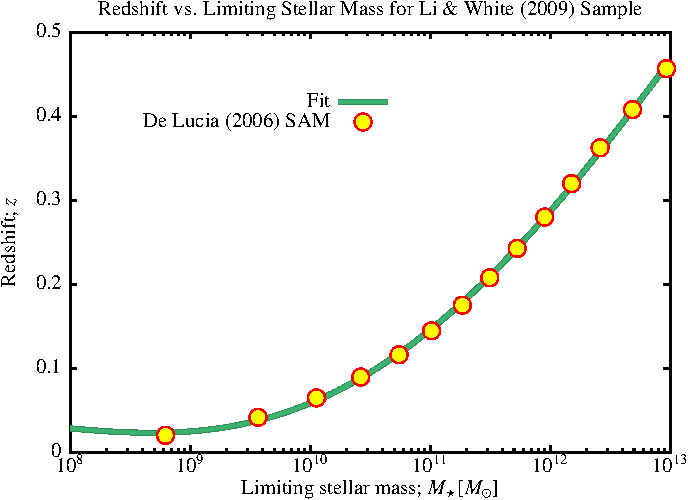
\includegraphics[width=85mm,trim=0mm 0mm 0mm 4mm,clip]{Plots/DataAnalysis/SDSSMassLuminosityRelation.pdf}
 \caption{The maximum redshift at which a galaxy of given stellar mass can be detected in the sample of \protect\cite{li_distribution_2009}. Points show the results obtained using the \protect\cite{de_lucia_hierarchical_2007} model from the Millennium Database, while the lines shows a polynomial fit to these results (given in eqn.~\ref{eq:DepthPolynomial}).}
 \label{fig:SDSSDepthFit}
\end{figure}

\subsection{Martin et al. (2010)}

Selected with {\tt surveyGeometryMethod}$=${\tt Martin-2010-ALFALFA}, this method describes the survey geometry of \cite{martin_arecibo_2010}. 

For the angular mask we use the three disjoint regions defined by 07$^{\rm h}$30$^{\rm m}$ $<$ R.A. $<$ 16$^{\rm h}$30$^{\rm m}$, +04$^\circ$ $<$ decl. $<$ +16$^\circ$, and +24$^\circ$ $<$ decl. $<$ +28$^\circ$ and 22$^{\rm h}$ $<$ R.A. $<$ 03$^{\rm h}$, +14$^\circ$ $<$ decl. $<$ +16$^\circ$, and +24$^\circ$ $<$ decl. $<$ +32$^\circ$ corresponding to the sample of \cite{martin_arecibo_2010}. When the survey window function is needed we generate randomly distributed points within this angular mask and out to the survey depth. These points are used to determine which elements of a 3D grid fall within the window function.

To estimate the depth of the \cite{martin_arecibo_2010} sample as a function of galaxy HI mass we first infer the median line width corresponding to that mass. To do so, we have fit the median line width-mass relation from the $\alpha.40$ sample with power-law function as shown in Fig.~\ref{fig:ALFALFALineWidthMassRelation}. We find that the median line width can be approximated by
\begin{equation}
 \log_{10} (W_{\rm 50}/\hbox{km s}^{-1}) = c_0 + c_1 \log_10(M_{\rm HI}/M_\odot),
 \label{eq:ALFALFALineWidthMassRelation}
\end{equation}
with $c_0=-0.770$ and $c_1=0.315$. Given the line width, the corresponding integrated flux limit, $S_{\rm int}$, for a signal-to-noise of $6.5$ is inferred using equation~(A1) of \cite{haynes_arecibo_2011}. Finally, this integrated flux limit is converted to maximum distance at which the source could be detected using the expression given in the text of section~2.2 of \cite{martin_arecibo_2010}:
\begin{equation}
 M_{\rm HI} = 2.356\times10^5 \left({D\over \hbox{Mpc}}\right)^2 \left({S_{\rm int}\over\hbox{Jy km s}^{-1}}\right).
\end{equation}

\begin{figure}
 \includegraphics[width=85mm,trim=0mm 0mm 0mm 4mm,clip]{Plots/DataAnalysis/ALFALFAHIMassFunctionLineWidthMassRelation.pdf}
 \caption{HI line width vs. HI mass as measured from the $\alpha.40$ survey of \protect\cite{martin_arecibo_2010}. Red points with error bars show individual measurements, while the larger circles indicate the running median of these data. The green line is a power-law fit to the running median as described in eqn.~(\protect\ref{eq:ALFALFALineWidthMassRelation}).}
 \label{fig:ALFALFALineWidthMassRelation}
\end{figure}
